\chapter{Capacitively Coupled Pixel Detectors for the CLIC Vertex Detector}
\label{chap:theory}

\chapterquote{There, sir! that is the perfection of vessels!}
{Jules Verne, 1828--1905}

%========================================================================================
%========================================================================================

\section{Introduction}
Identification of heavy-flavour quarks and tau-leptons relies upon precise reconstruction of the secondary displaced vertices produced in the decay of these particles, in addition to the accurate association of daughter tracks to those vertices.  For the CLIC vertex detector a very high spatial resolution of approximately 3 {\mu}m, as well as good geometric coverage extending to low $\theta$ values, are essential for achieving the precision on the reconstructed vertices necessary for identification of heavy-flavour quarks and tau-leptons.  The vertex detector must also have a low material budget (less than 0.2 $\text{X}_{0}$ per layer) in order to prevent additional decay vertices due to material interactions (CONFIRM!), and maintain a low occupancy, despite the high presence of beam-induced background particles. This will be achieved by the use of time-tagging, to an accuracy of 10 ns, to identify particles produced around the physics event of interest.  

As there are currently no technology options that have fulfilled all of the criteria for the CLIC vertex detector, the CLIC experiment has developed a wide R\&D program to consider  new technologies that could be of use in the vertex detector. High-voltage complementary metal-oxide-semiconductor (HV-CMOS) sensors, capacitively coupled to a separate readout ASIC are one such option. The performance of prototype detectors for CLIC, and the impact of mechanical tolerances that are present in their manufacture, are presented.  

WILL YOU DISCUSS CAPACITIVE COUPLING IN YOUR THEORY CHAPTER? SOMETHING LIKE TRADITIONAL BUMP-BONDED DEVICES, ETC.? OTHERWISE LOTS OF CONCEPTS ARE ABSENT HERE. OK, JUST SAW THE NEXT SECTION... 

%========================================================================================

\subsection{HV-CMOS}

Pixel detectors can be broadly classified in two distinct groups: hybrid detectors, where a separate sensor and readout chip are bonded together; and fully-integrated devices, where the collection diode is implanted in the same piece of silicon as the readout circuitry. This latter approach has traditionally not been suitable for applications with high timing requirements, due to the relatively slow charge collection time and limited on-pixel functionality. Developments in CMOS technologies in recent years have, however, led to many new detector designs which may overcome some of these issues. 

ACTUALLY, DO YOU PLAN IN YOUR THEORY SECTION TO DISCUSS SILICON TECHNOLOGY? SHOULD YOU EXPLAIN COLLECTION DIODE, PN JUNCTION, ETC?

HV-CMOS is a processing technology whereby the n-MOS and p-MOS transistors forming the on-pixel electronics are placed entirely within a deep n-well (shown in  \ref{fig:hvcmos}), which acts as the charge collection diode as well as shielding the circuitry from the p-substrate. This shielding allows the application of a moderate bias voltage to the sensor bulk, producing a depletion region that facilitates fast charge collection (unlike conventional MAPS). This has the additional benefit of preventing competition for the charge collection, as is the case for conventional MAPS where n-wells from both the collection diode and PMOS transistors may collect deposited charge.

\begin{figure}
\centering
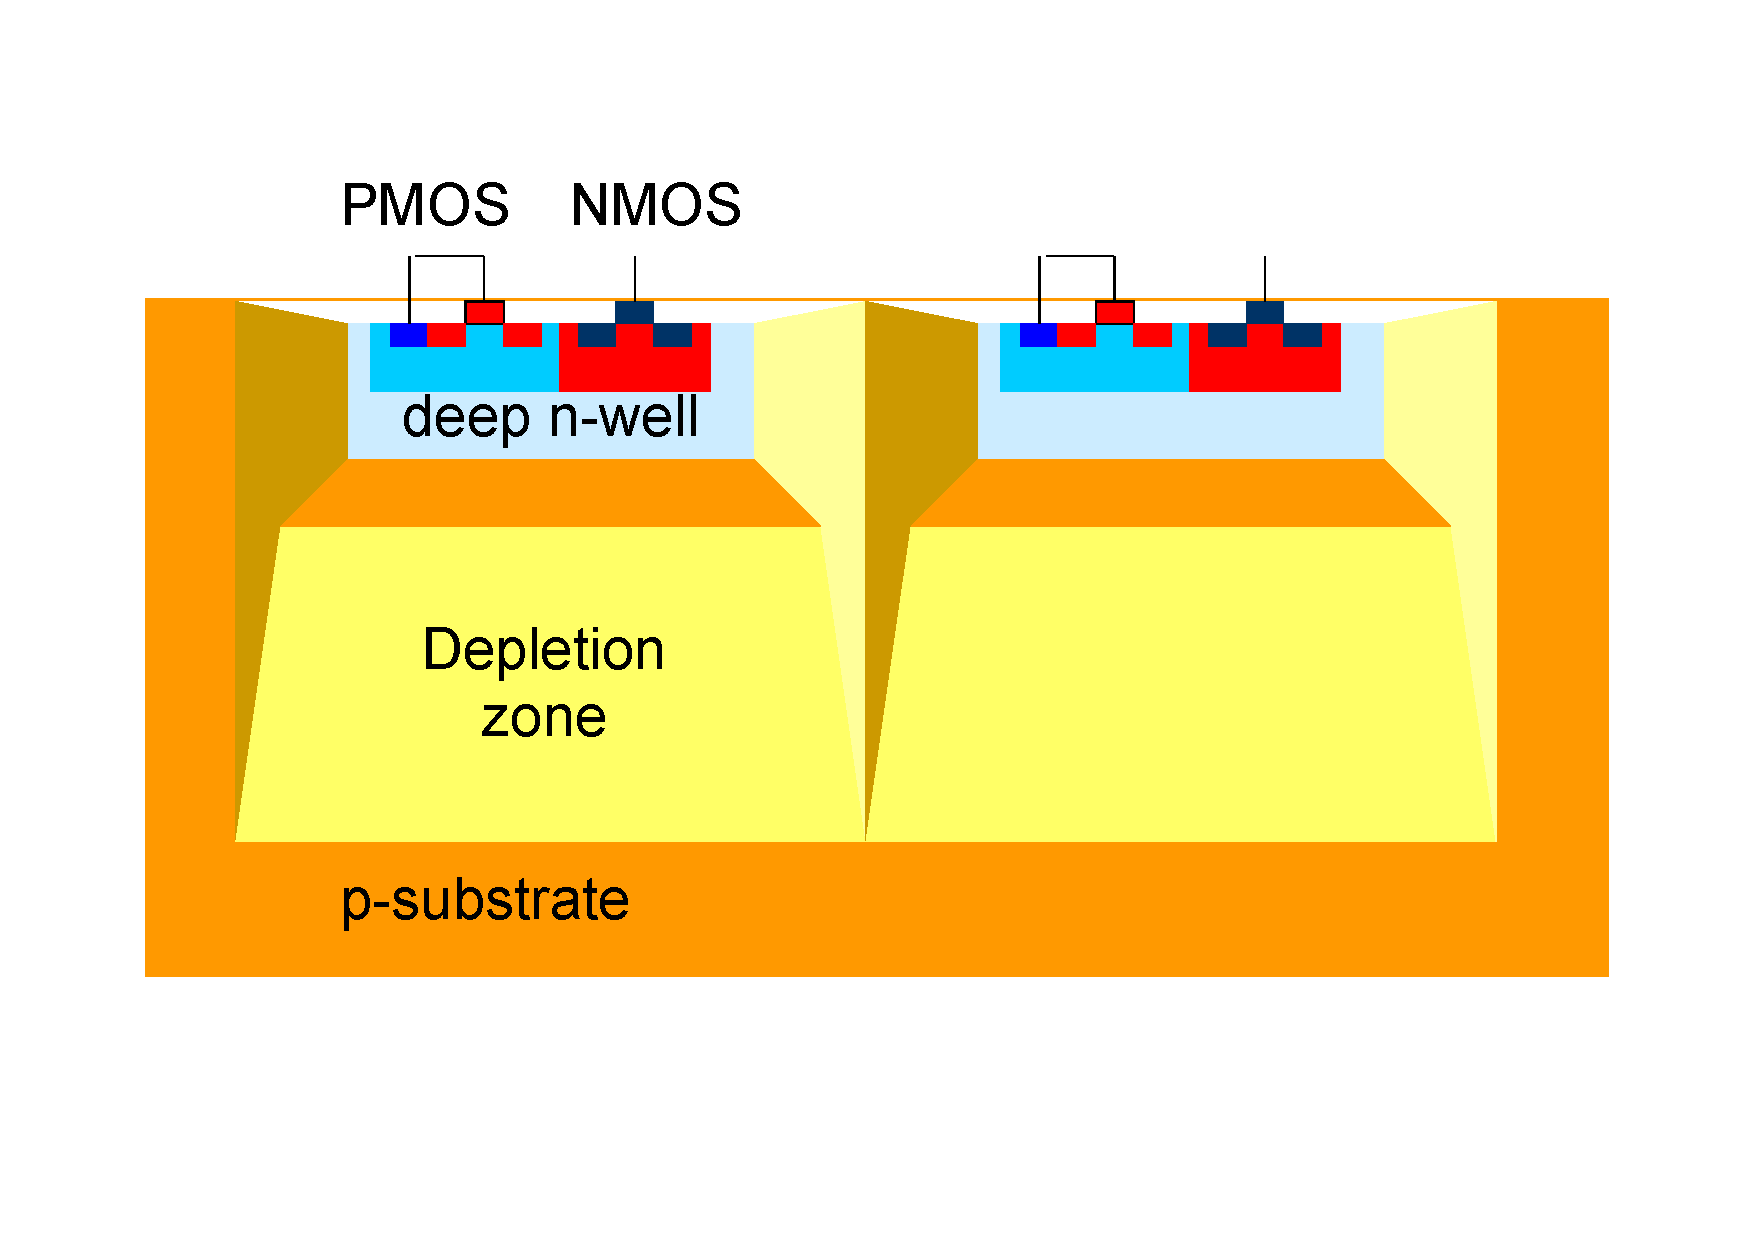
\includegraphics[width=0.75\textwidth]{CLICdpVertex/Plots/HV-CMOSDiagram.pdf}
\caption[HV-CMOS diagram.]{I NEED A BETTER DIAGRAM!}
\label{fig:hvcmos}
\end{figure}

While HV-CMOS offer the possibility of fast charge collection with integrated on-pixel functionality, several limitations still exist for this technology. Due to the requirement for all electronics to be placed inside the deep n-well, and the separation required between n-wells, only a limited physical area of the pixel is available for transistor layout. Additionally, due to the limited availability of quadruple-well technology, it is not possible to implement full CMOS logic inside the deep n-well without coupling the p-MOS transistors to the collection node, leading to noise injection. A relatively simple pixel architecture has thus been implemented, with a focus on producing a small-pitch device that can reach the requirements of the CLIC vertex detector. Given the issues involved in bump-bonding a hybrid pixel detector (detailed below), capacitive coupling of the HV-CMOS sensor to a dedicated readout ASIC has been pursued. This is only made possible by the implementation of an amplifier in the HV-CMOS pixel, allowing the small pixel capacitance to be overcome. A schematic approach of this can be see in figure \ref{fig:ccpdandclicpix}.
 
\begin{figure}
\centering
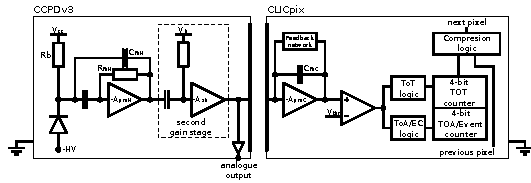
\includegraphics[width=1.0\textwidth]{CLICdpVertex/Plots/schematic.pdf}
\caption[Schematic of CCPDv3 and CLICpix pixels.]{Schematic of CCPDv3 and CLICpix pixels.}
\label{fig:ccpdandclicpix}
\end{figure}

%========================================================================================

\subsection{The CLICpix Readout ASIC}

The readout ASIC used in this study (REPHRASE? DEVELOPED FOR CLIC?) is the CLICpix, a hybrid pixel readout chip with pixels containing a charge-integrating amplifier connected to a discriminator, as shown in figure \ref{fig:ccpdandclicpix}.  The discriminator fires for as long as the input signal is over a given threshold, and is used as the input for further logic operations to record the time of arrival and magnitude of the collected charge, using a Time over Threshold (ToT) measurement. The ToT is stored in a 4-bit on-pixel counter.  The CLICpix ASIC operates using a shutter-based readout, where the entire matrix is kept active while the shutter is open and when closed the matrix is readout in its entirety.  This is designed in order to match the expected beam structure for the CLIC experiment, as the accelerator will deliver bunch trains of $e^{+}$ and $e^{-}$ that are separated by 20~ms.  Each bunch train contains 312~bunches with a spacing of 0.5~ns, giving a total train length of 156~ns.  

Due to variations in the manufacturing process, the threshold voltage seen by each CLICpix pixel is slightly different, which if not accounted for results in a threshold dispersion across the matrix. To suppress these fluctuations, each CLICpix pixel contains a 4-bit local adjustment to the threshold voltage, to unify the response of the detector. The threshold equalisation is achieved by performing two threshold scans of the matrix, once with all four bits set to 0 (no local threshold adjustment), and a second time with all four bits set to 1 (maximum local threshold adjustment). For each scan, the baseline voltage of each pixel is determined. By applying a linear interpolation between the 0000 and 1111 cases, each pixel can be tuned to a common point, such that all pixels respond at the same global threshold.

COULD CHANGE THIS SECTION TO "CLIC ASICS" AND THEN ADD SOME DESCRIPTION OF THE CCPDv3, AND ADDING SOME GENERAL FEATURES LIKE 25 UM PITCH AND 64*64 PIXELS, WHICH DON'T FIT IN WELL BELOW.

%========================================================================================

\subsection{Capacitive Coupling}

Solder bump-bonding is the typical method that is used for hybrid pixel detectors to connect the sensor to the readout ASIC, however bump-bonding is both expensive and sets limits on the thickness of both objects for mechanical stability.  An alternative to this involves using a thin layer of glue to form a capacitive connection between the active sensor and the readout ASIC.  While this procedure reduces the cost and material budget with respect to bump-bonding, it has only recently been used to produce prototype detectors and as such, detailed studies must be carried out. (REPHRASE A LITTLE THOUGH...)

%========================================================================================

\section{Construction}

Two of the main issues involved in constructing capacitively coupled pixel detectors are the uniformity of the glue layer achieved and the physical alignment between the pads on the active sensor and the readout ASIC. While the former has been investigated in another study (CITE STUDY), the latter will be presented below. For this work, a number of pixel detectors were constructed that contained misalignments between the HV-CMOS and CLICpix coupling pads (as shown in figure \ref{fig:alignment}), in order to quantify the impact on the detector performance. Table \ref{table:alignment} contains a summary of the samples studied.

\begin{figure}
\centering
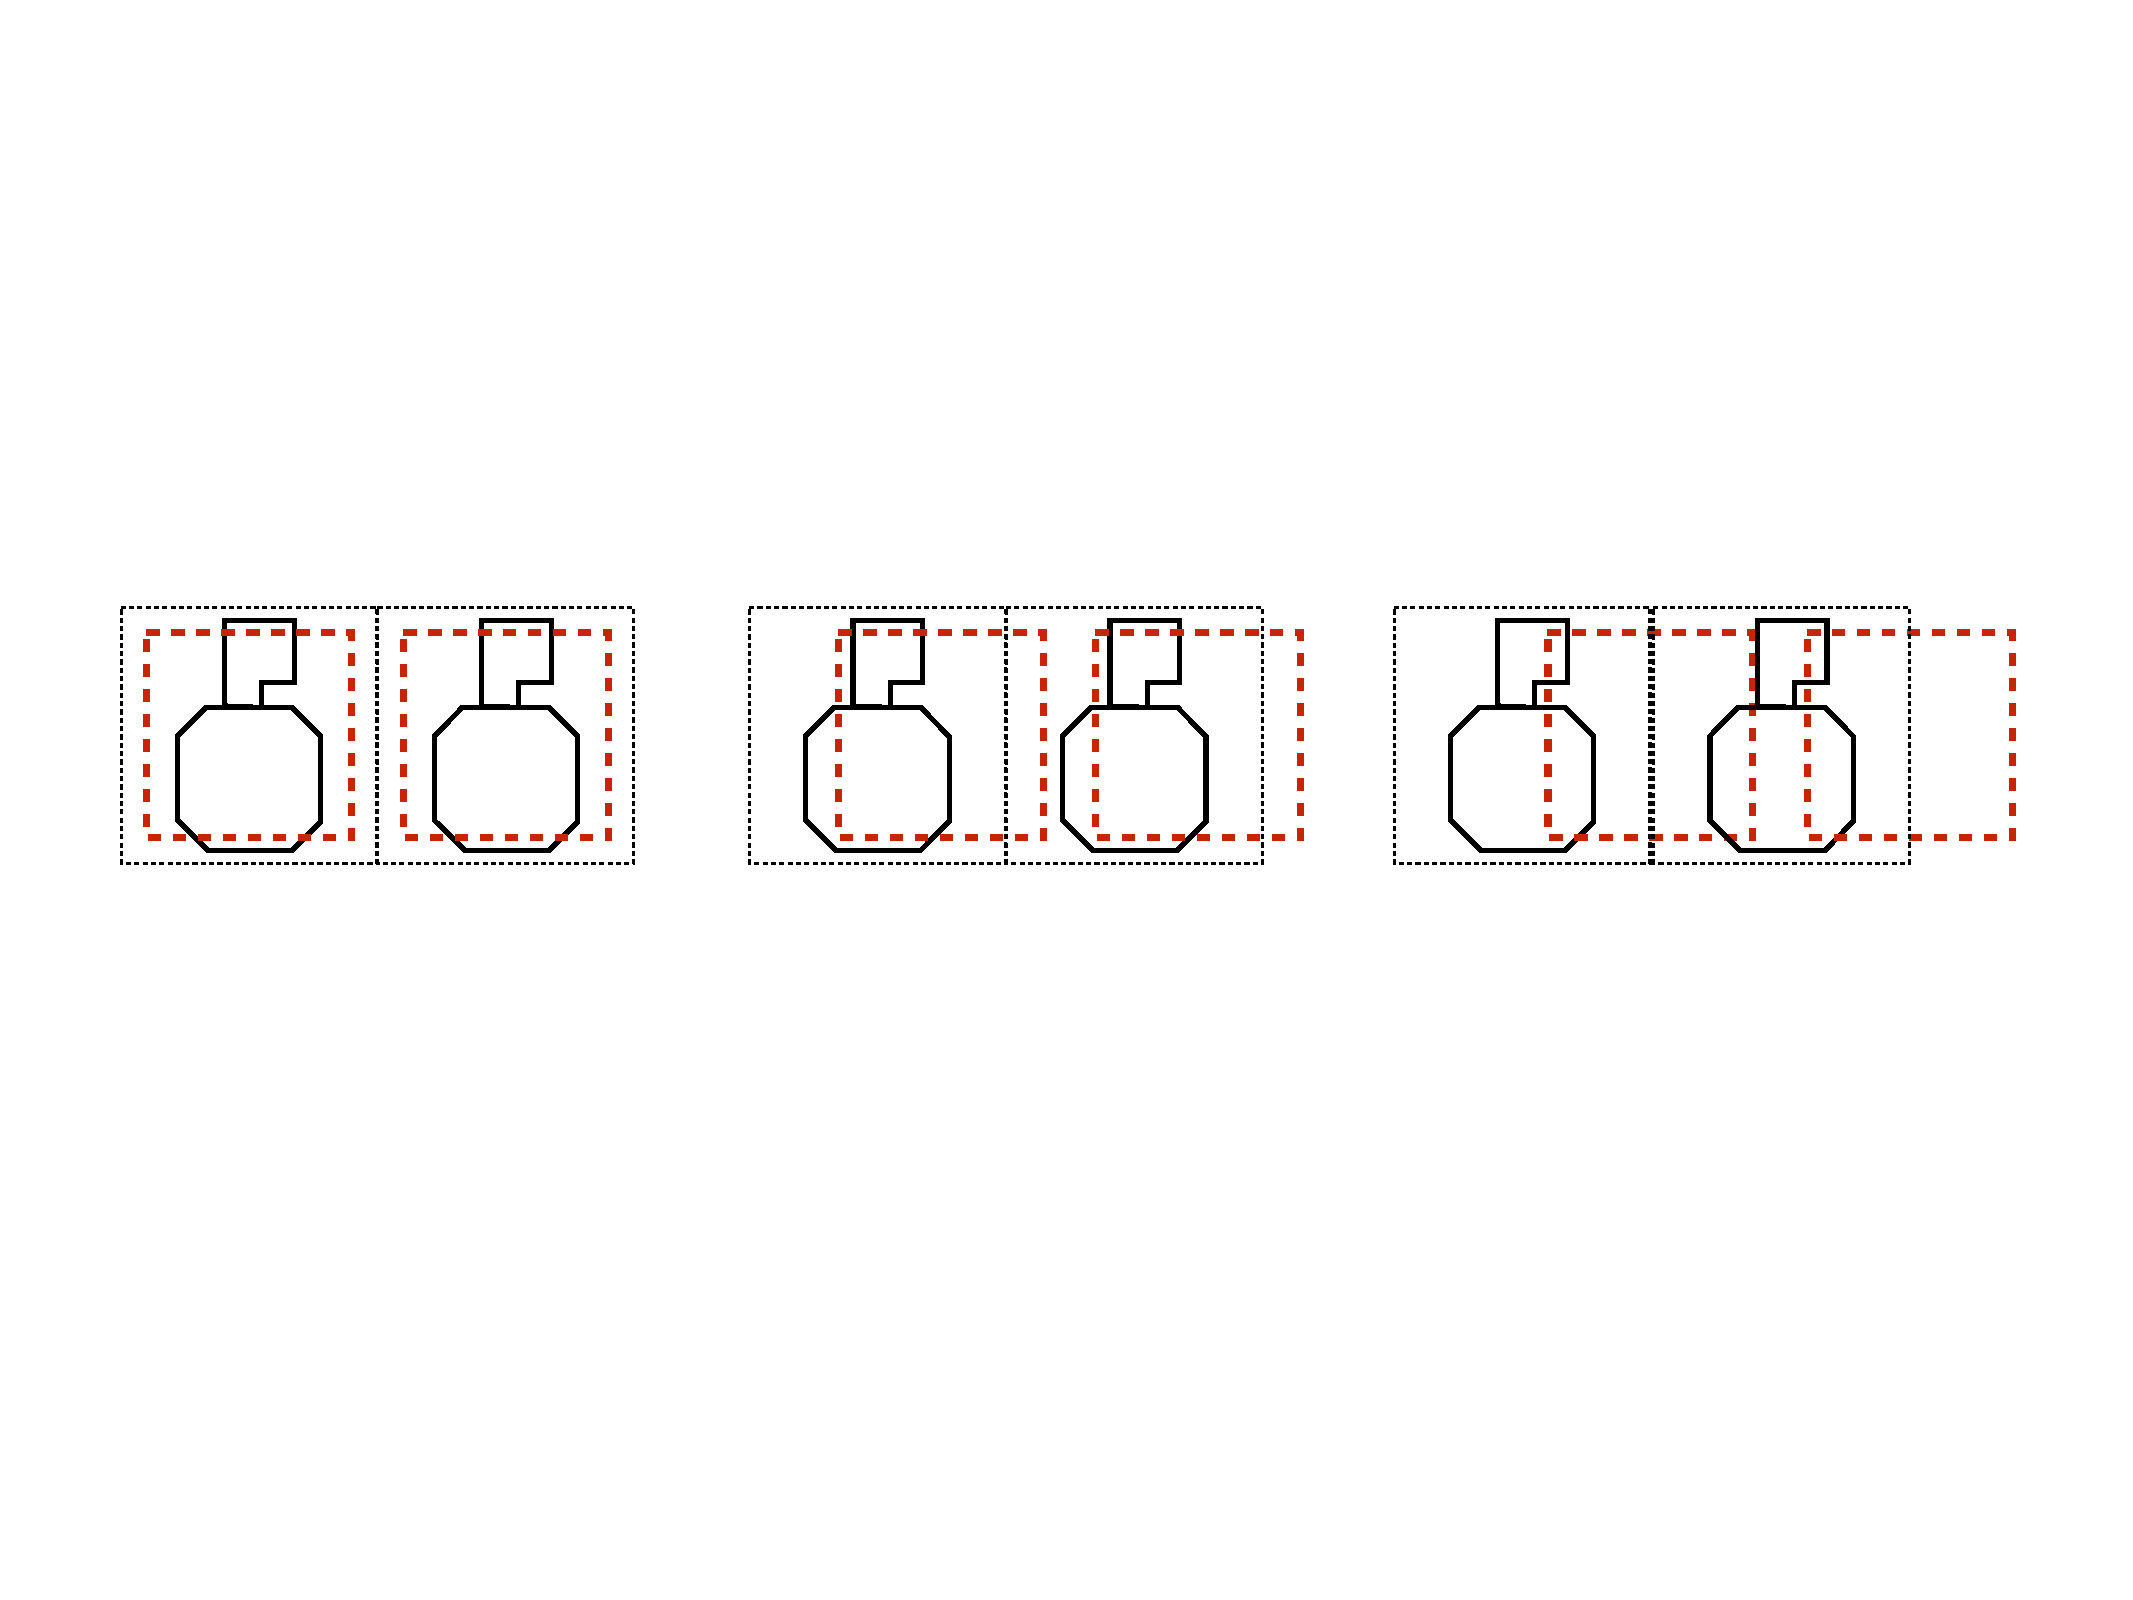
\includegraphics[width=1.0\textwidth]{CLICdpVertex/Plots/misalignedPads.pdf}
\caption[Schematic of alignment of CCPDv3 and CLICpix sensors studied in this analysis.]{Alignment schematic of the CCPDv3 + CLICpix detectors studied.  The red dotted line represents the CCPDv3 pad and the solid black line represents the CLICpix top metal layer.  From left to right; centred pixels, 1/4 offset (6.25 {\mu}m) and 1/2 offset (12.5 {\mu}m).}
\label{fig:alignment}
\end{figure}

\begin{table}[h!]
\centering
\begin{tabular}{ l l }
\hline
Assembly & Alignment \\ 
\hline
SET9 & Centred \\
SET10 & $\frac{1}{4}$ Offset \\
%SET11 & $\frac{1}{2}$ Offset \\
SET12 & Centred \\
SET13 & Centred \\
SET14 & $\frac{1}{2}$ Offset REMOVED, NO?\\
SET15 & Centred \\
SET16 & $\frac{1}{2}$ Offset \\
\hline
\end{tabular}
\caption[A list of the detectors considered in this study, showing the misalignment of the HV-CMOS and CLICpix coupling pads.]{A list of the detectors considered in this study, showing the misalignment of the HV-CMOS and CLICpix coupling pads.}
\label{table:alignment}
\end{table}

%The pitch of the sensors, both the HV-CMOS active pixel sensor and CLICpix readout ASIC, produced for this study was 25 {\mu}m and the matrix size was 64$\times$64. 

The full details of the glueing process can be found in [CERN NOTE CITE], along with a study of the absolute precision of the manufacturing procedure.  It was found that for devices constructed in an identical fashion to those considered here, the glue layer thicknesses were less than 1~{\mu}m and the precision on the pad positioning was less than 0.5~{\mu}m.  

%========================================================================================
%========================================================================================

\section{Device Characterisation}

%========================================================================================

The assemblies were characterised using a series of lab experiments as well as in realistic experimental conditions using the CERN SPS test beam.  Due to the complexities of testing assemblies in a test beam, extensive lab test were performed first to characterise as many properties of the assemblies as possible.  The lab experiments performed were as follows:

\begin{itemize}
\item \textbf{Radioactive source measurements}.  The goal of this measurement is to examine both the output of the HV-CMOS voltage and the response of the CLICpix readout chip when a radioactive source is used to deposit charge within the HV-CMOS sensor.  
\item \textbf{Test pulse calibration of the CLICpix chip}.  The goal of this measurement is to calibrate the response of the CLICpix sensor.  This is achieved by injecting a voltage pulse of fixed height directly into the input of the chip and examining the output response.  
\end{itemize} 

%========================================================================================

\subsection{Source Measurements}
A radioactive source was used to deposit charge within the HV-CMOS sensor and used to characterise the response of the whole assembly.  The HV-CMOS sensor converts the deposited charge into a voltage, which in turn passes through the capacitively coupled glue layer and into the CLICpix chip.  Measurements were made of the output voltage produced by the HV-CMOS and the response of the CLICpix readout chip, in units of ToT.  As the exact amount of charge deposited by the radioactive sources is unknown, this experiment focuses on examining the form of the voltage signal produced by the HV-CMOS and determining the response of the CLICpix chip as a function of this voltage.  As the HV-CMOS signal must pass through the capacitively coupled glue layer before being measured by the CLICpix chip, this experiment characterises the behaviour of the gluing layer as well as the sensor and readout chips.

%========================================================================================

\subsubsection{Experimental Setup}
In order to characterise the samples, a $\text{Sr}^{90}$ radioactive source was used to deposit charge in the HV-CMOS sensor. $\text{Sr}^{90}$ undergoes $\beta^{-}$ decay to form $\text{Y}^{90}$, which in turn undergoes $\beta^{-}$ decay to form the stable isotope $\text{Z}^{90}$.  Each $\beta^{-}$ decay produces an $\text{e}^{-}$ and a $\bar{\nu_{e}}$, with the $\text{e}^{-}$ used to deposit charge in the HV-CMOS sensing layer.  The $\text{Sr}^{90}$ source used for this experiment had an activity of 29.6 MBq.  

The radioactive source was positioned directly above the back-side of the HV-CMOS sensor, and measurements were made of both the ToT output from the CLICpix and the HV-CMOS analogue signal for individual pixels on the sensor.  The HV-CMOS pulse shape was recorded on a fast sampling oscilloscope that was also used to trigger the CLICpix readout.  The on-pixel event counter was used to veto events where multiple hits occurred within the active shutter period.  

\begin{figure}
\centering
\subfloat[]{\label{fig:pulseshape1}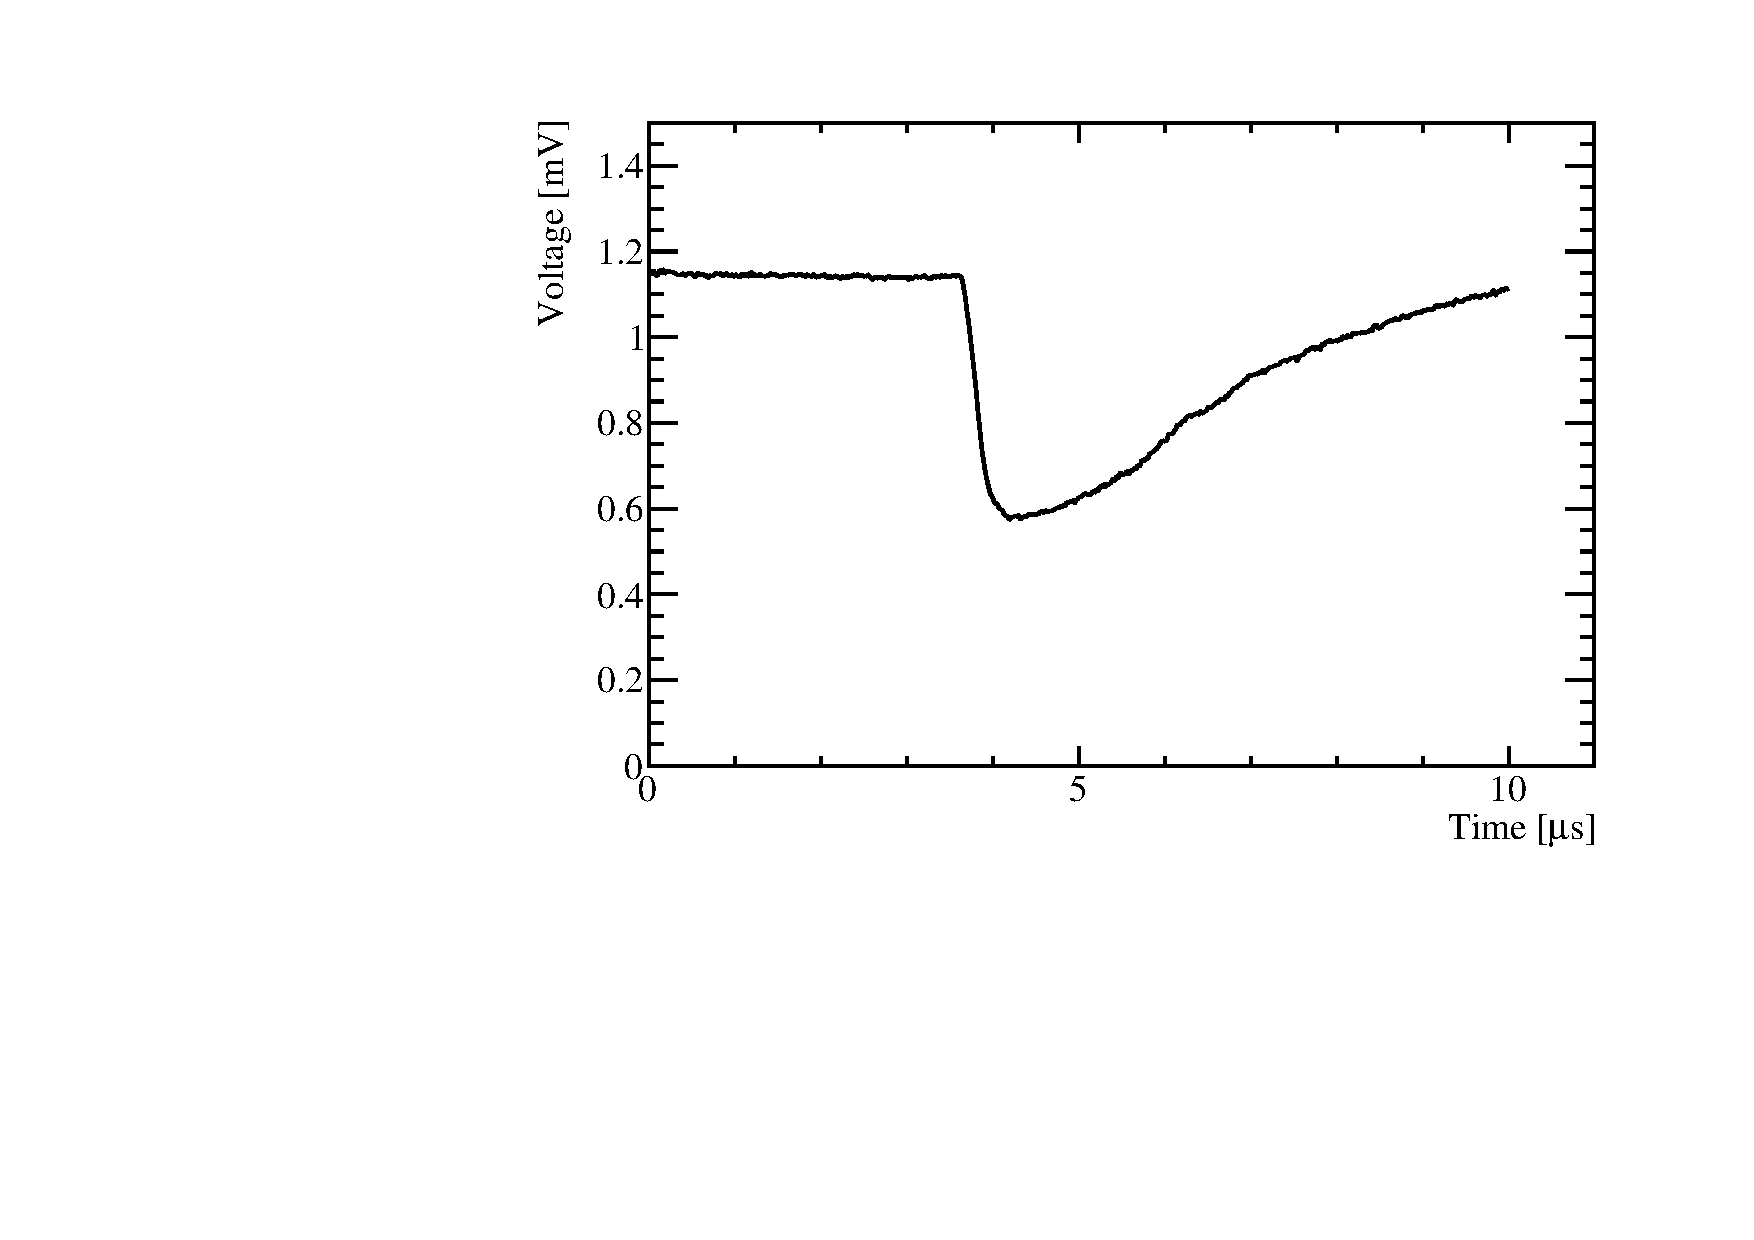
\includegraphics[width=0.5\textwidth]{CLICdpVertex/Plots/HV-CMOS/Frames/PulseShape01000NoOffset.pdf}}
\subfloat[]{\label{fig:pulseshape2}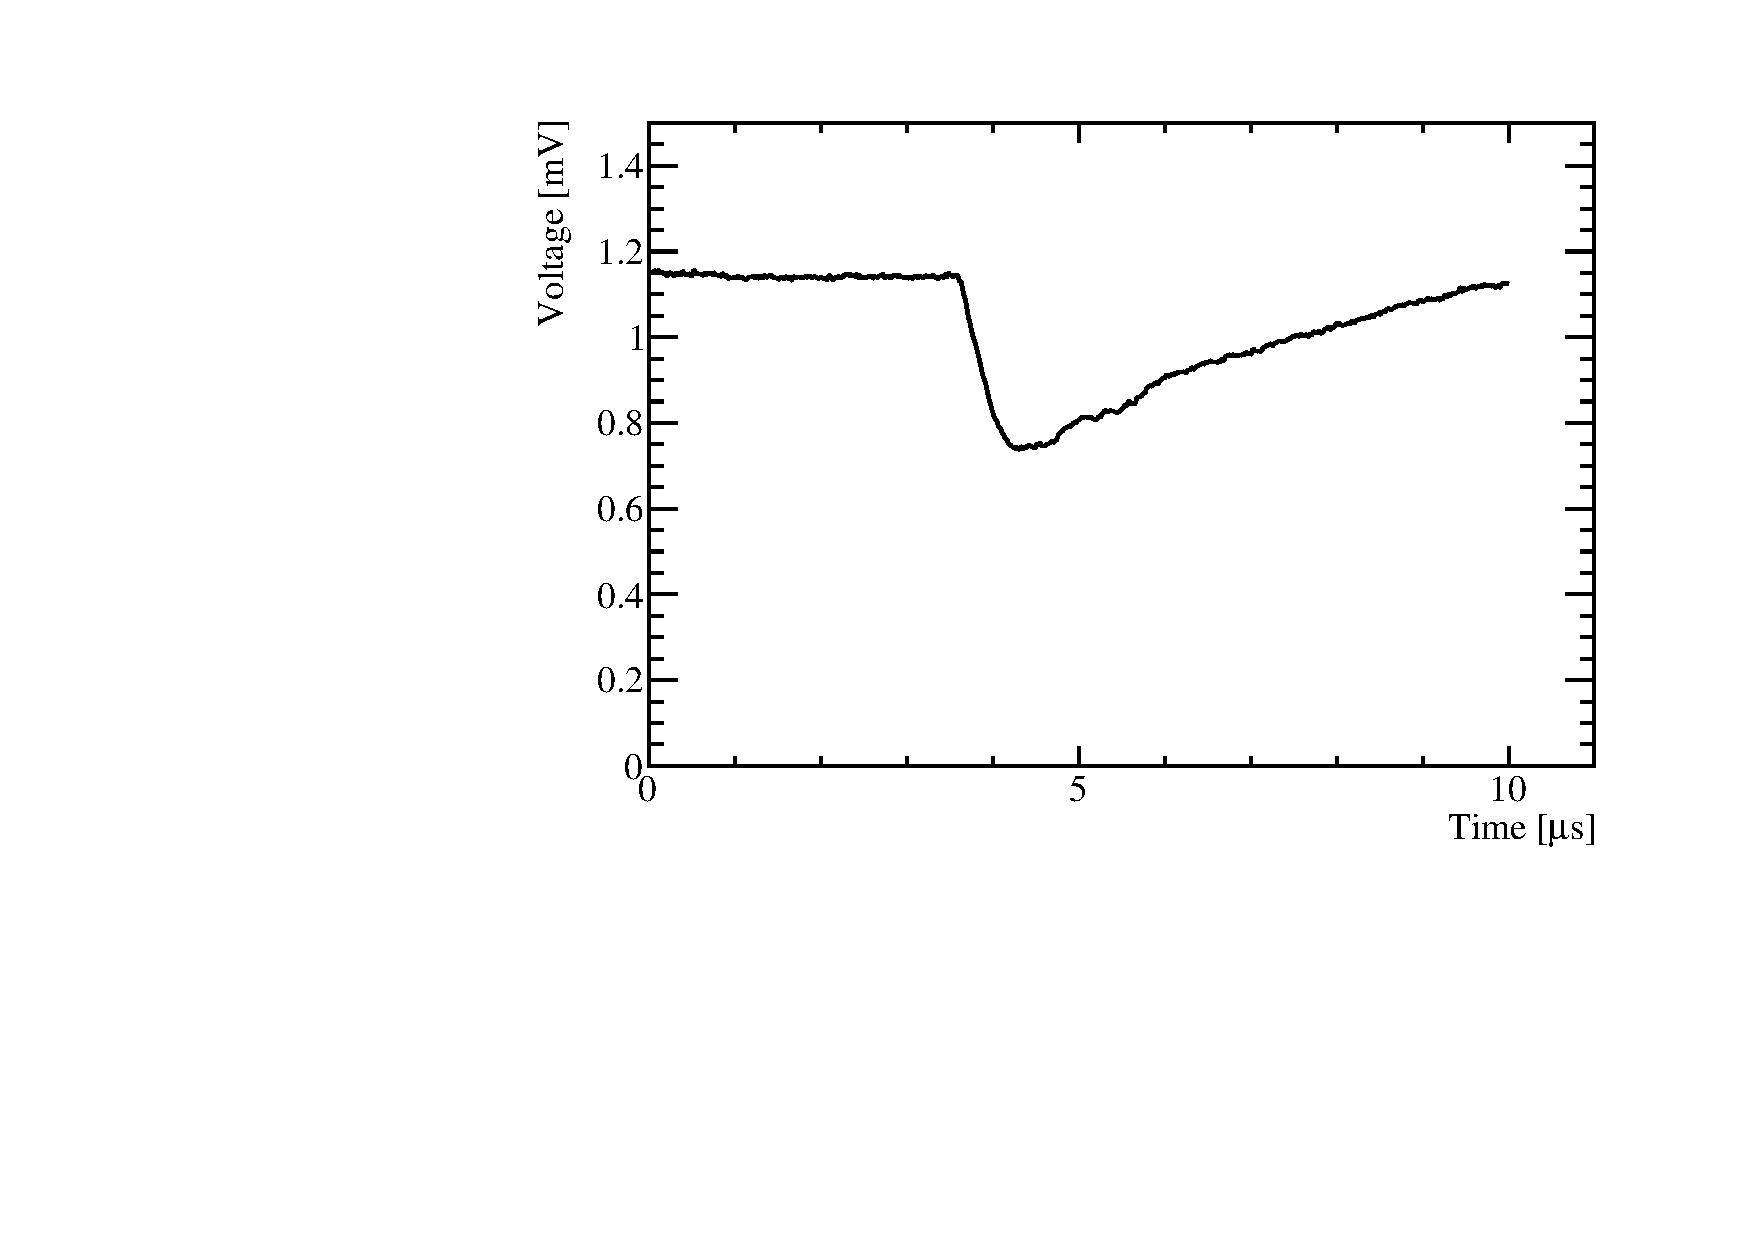
\includegraphics[width=0.5\textwidth]{CLICdpVertex/Plots/HV-CMOS/Frames/PulseShape01005NoOffset.pdf}}\hfill
\subfloat[]{\label{fig:pulseshape3}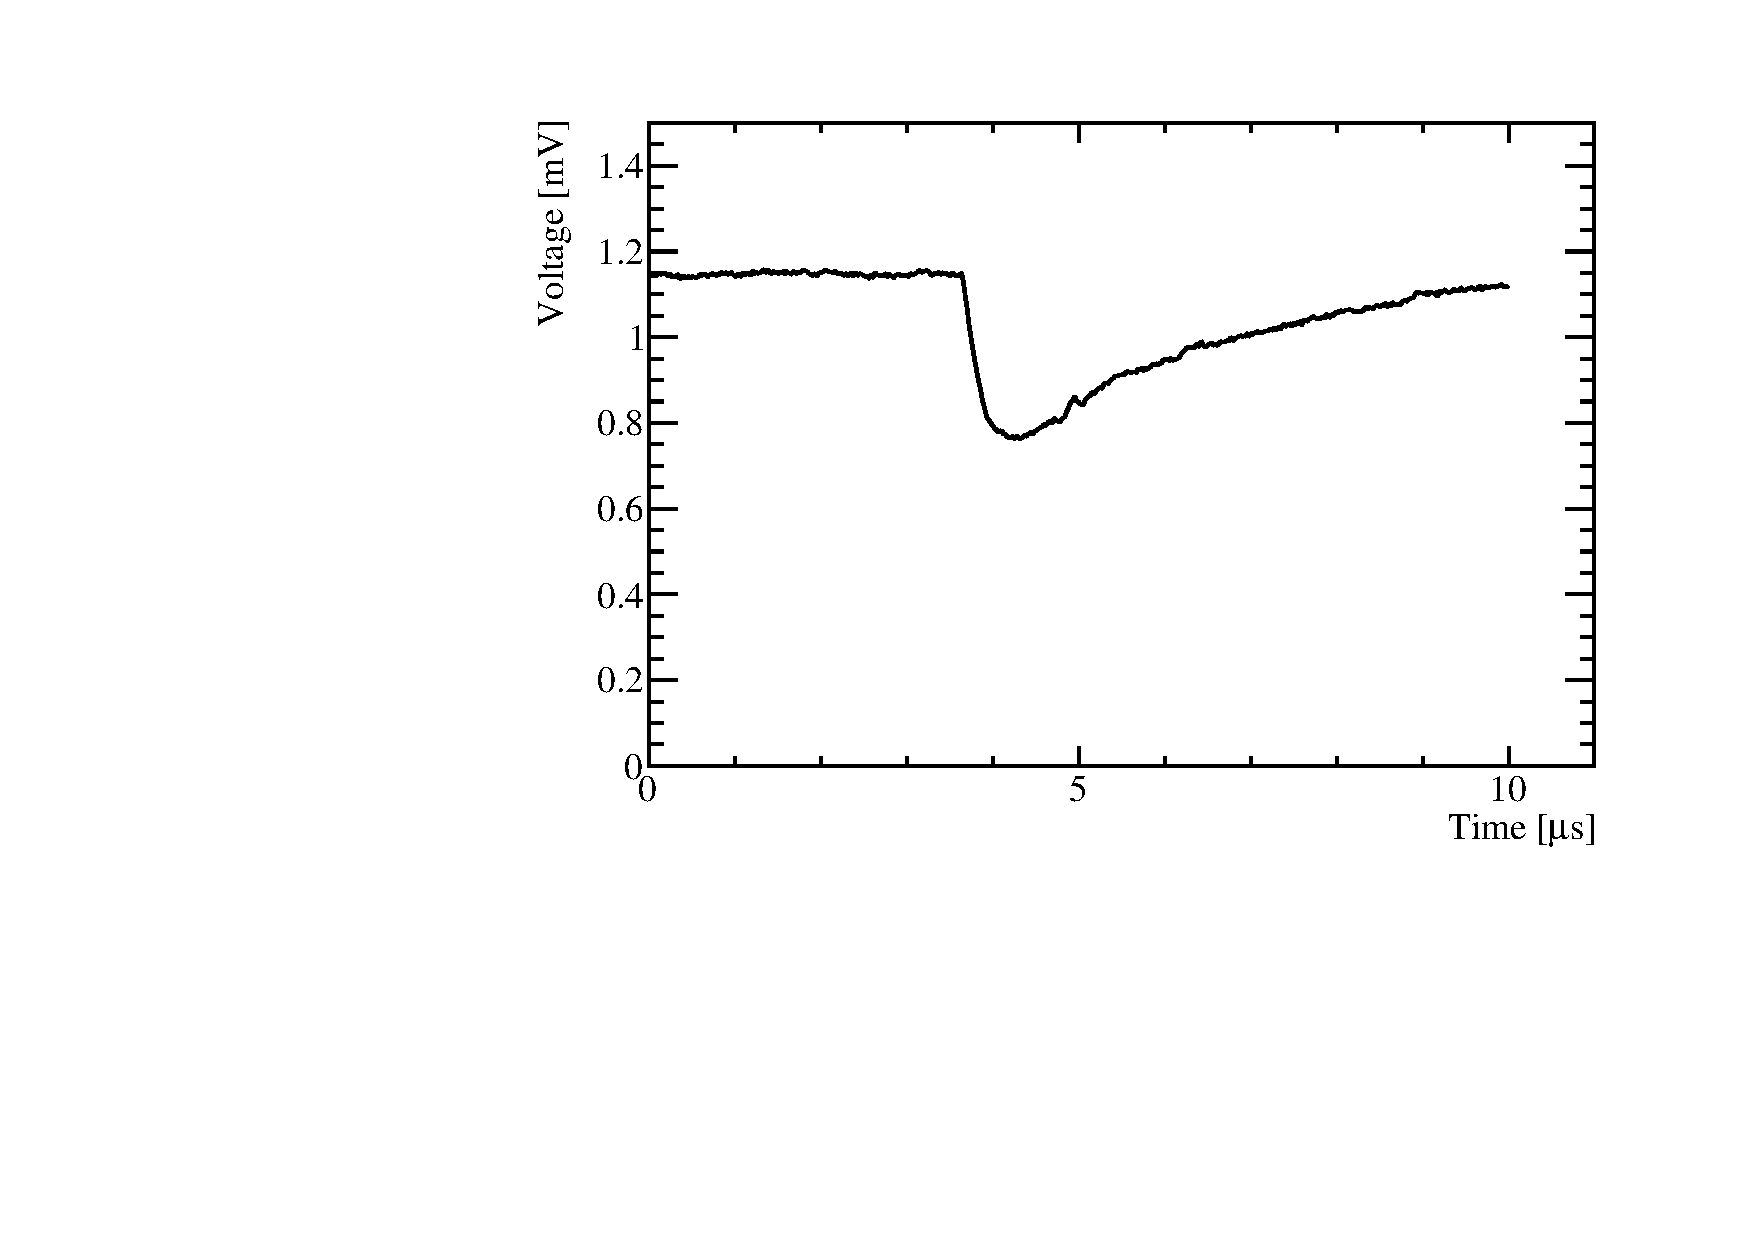
\includegraphics[width=0.5\textwidth]{CLICdpVertex/Plots/HV-CMOS/Frames/PulseShape01006NoOffset.pdf}}
\subfloat[]{\label{fig:pulseshape4}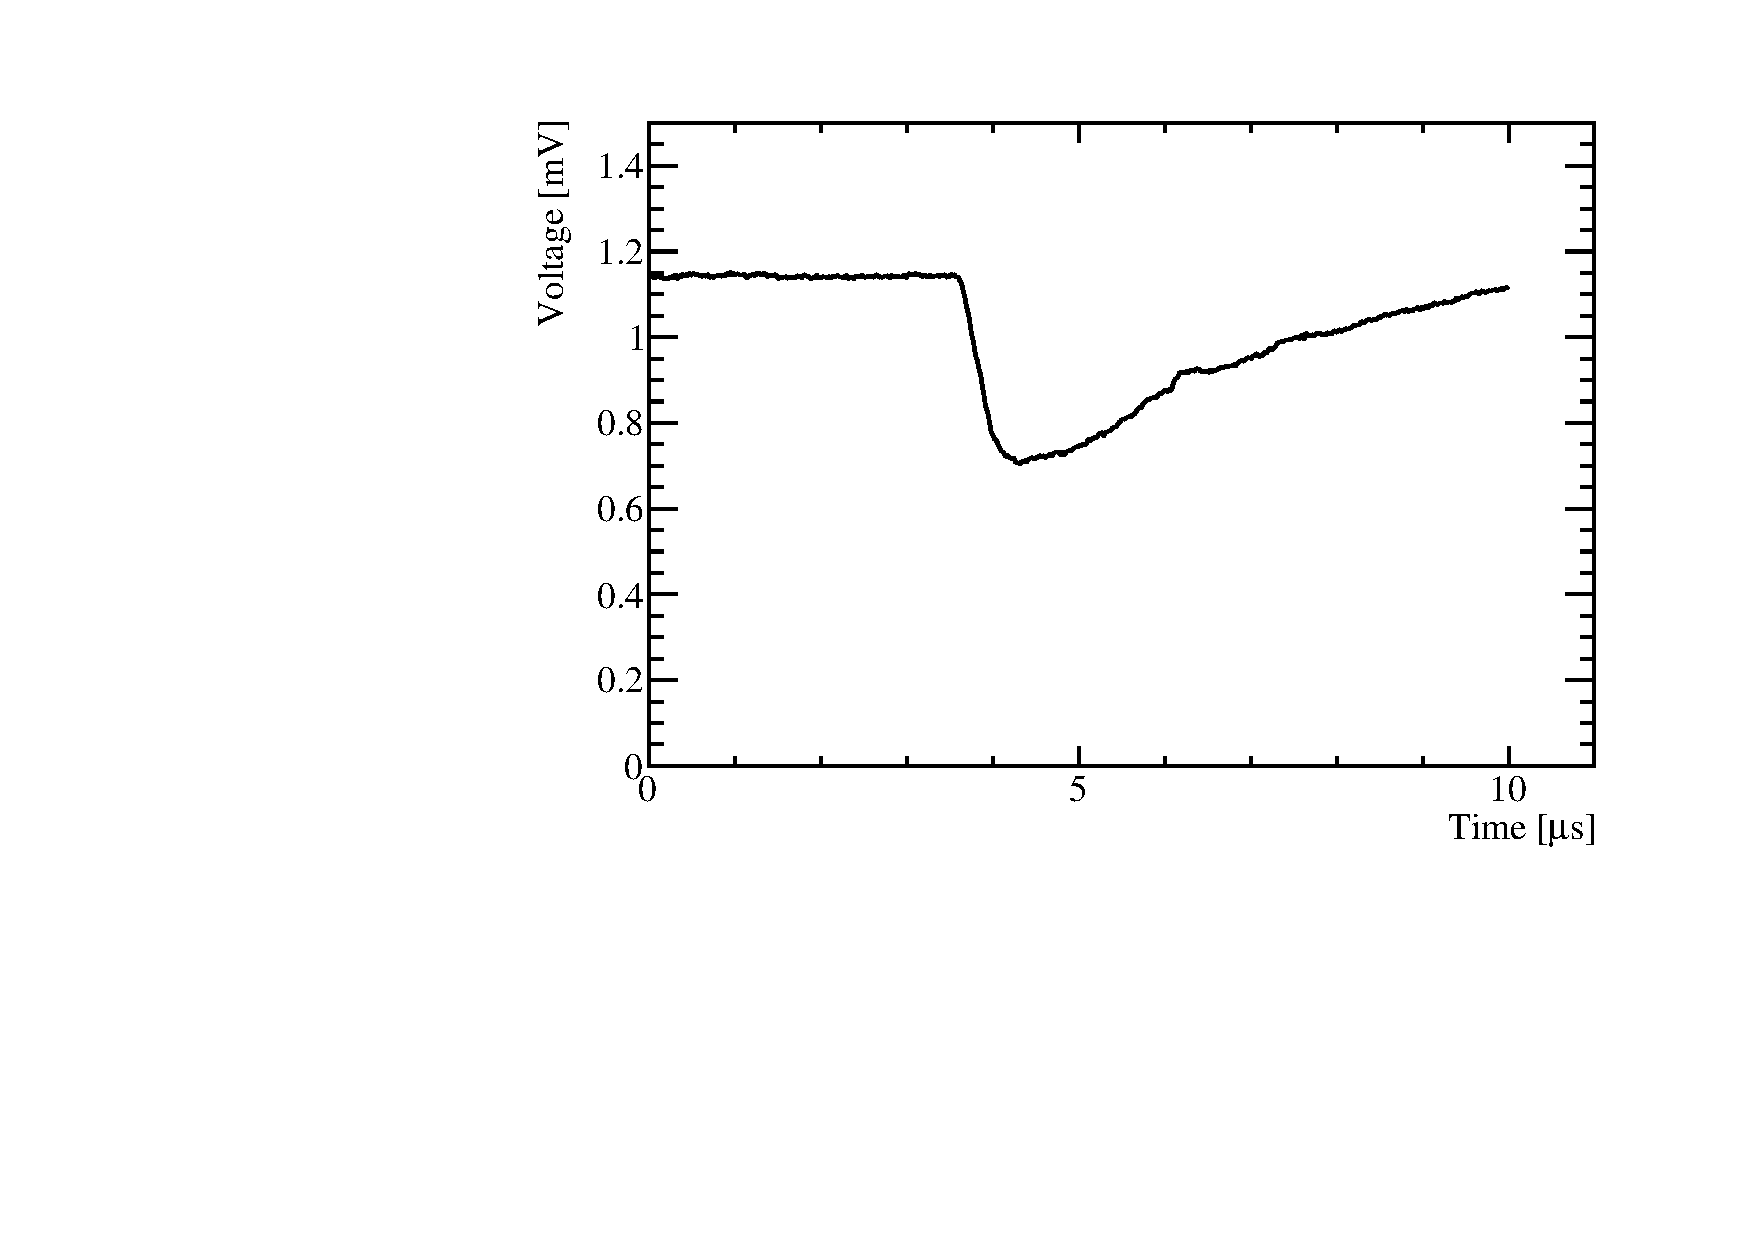
\includegraphics[width=0.5\textwidth]{CLICdpVertex/Plots/HV-CMOS/Frames/PulseShape01008NoOffset.pdf}}
\caption[HV-CMOS voltage pulses produced by radioactive $\text{Sr}^{90}$ source.]{HV-CMOS voltage pulses produced by radioactive $\text{Sr}^{90}$ source.}
\label{fig:pulseshapes}
\end{figure}

The HV-CMOS sensor was biased to 60~V during this experiment.  The analogue output has a baseline voltage of $\approx 1.15$~V, with signal saturation around a height of 700~mV.  Examples of the HV-CMOS output can be seen in figure \ref{fig:pulseshapes}.

%========================================================================================

\subsubsection{Analysis}

The quantities of interest related to the HV-CMOS output are the pulse height and rise time.  The baseline voltage was subtracted from the HV-CMOS analogue output and the pulse height inverted before the following analysis was applied.

\begin{figure}
\centering

\subfloat[\textbf{Rise time determination.}  The blue arrows show the change in time and voltage as the pulse goes from 10\% to 90\% of the raw pulse height.  This time is used as the definition of the rise time in the subsequent analysis.]{\label{fig:pulseshapeanalysistime}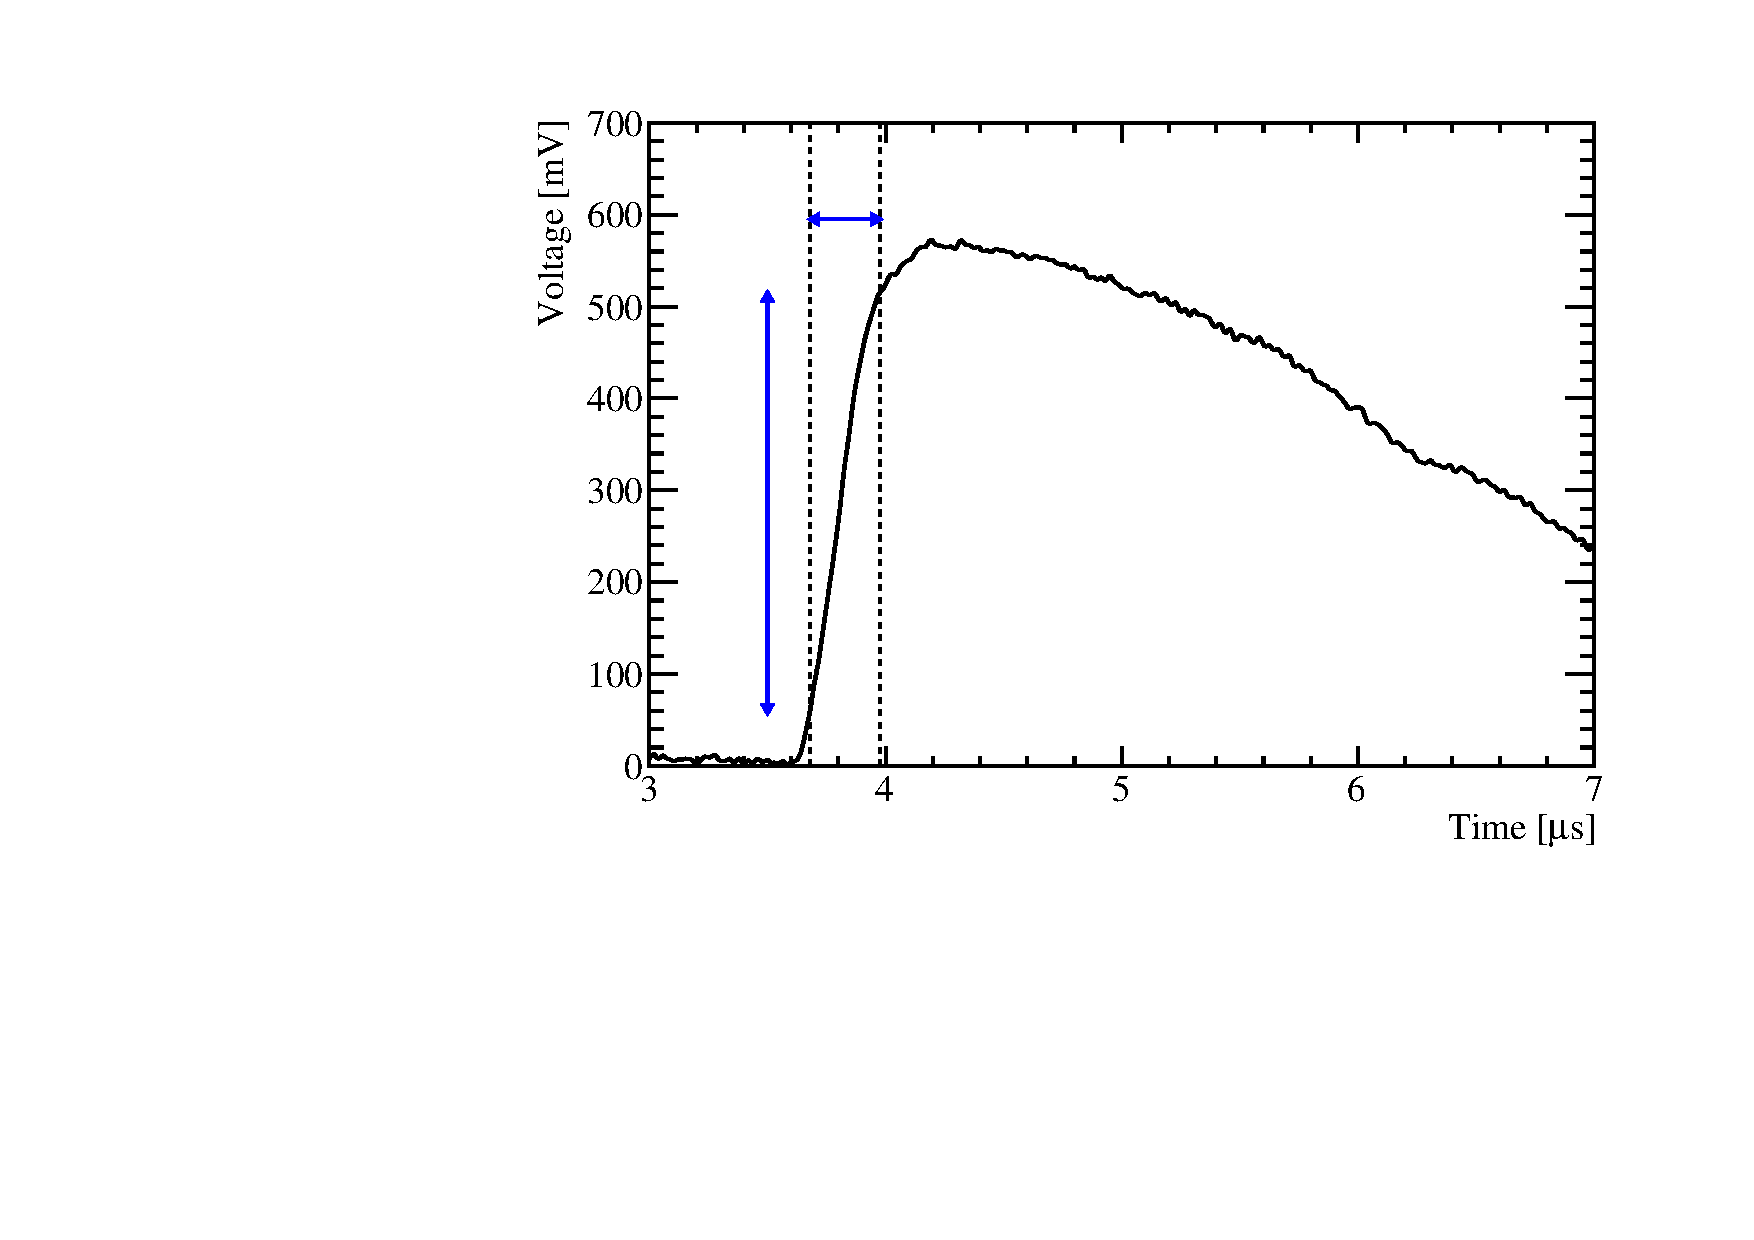
\includegraphics[width=0.5\textwidth]{CLICdpVertex/Plots/HV-CMOS/Frames/PulseShape01000FittingRiseTime.pdf}}

\subfloat[\textbf{Pulse height determination.} The red dotted line is a Gaussian fit to the peak of the pulse.  The peak is defined as the section of the signal above 90\% of the raw pulse height.]{\label{fig:pulseshapeanalysisvoltage}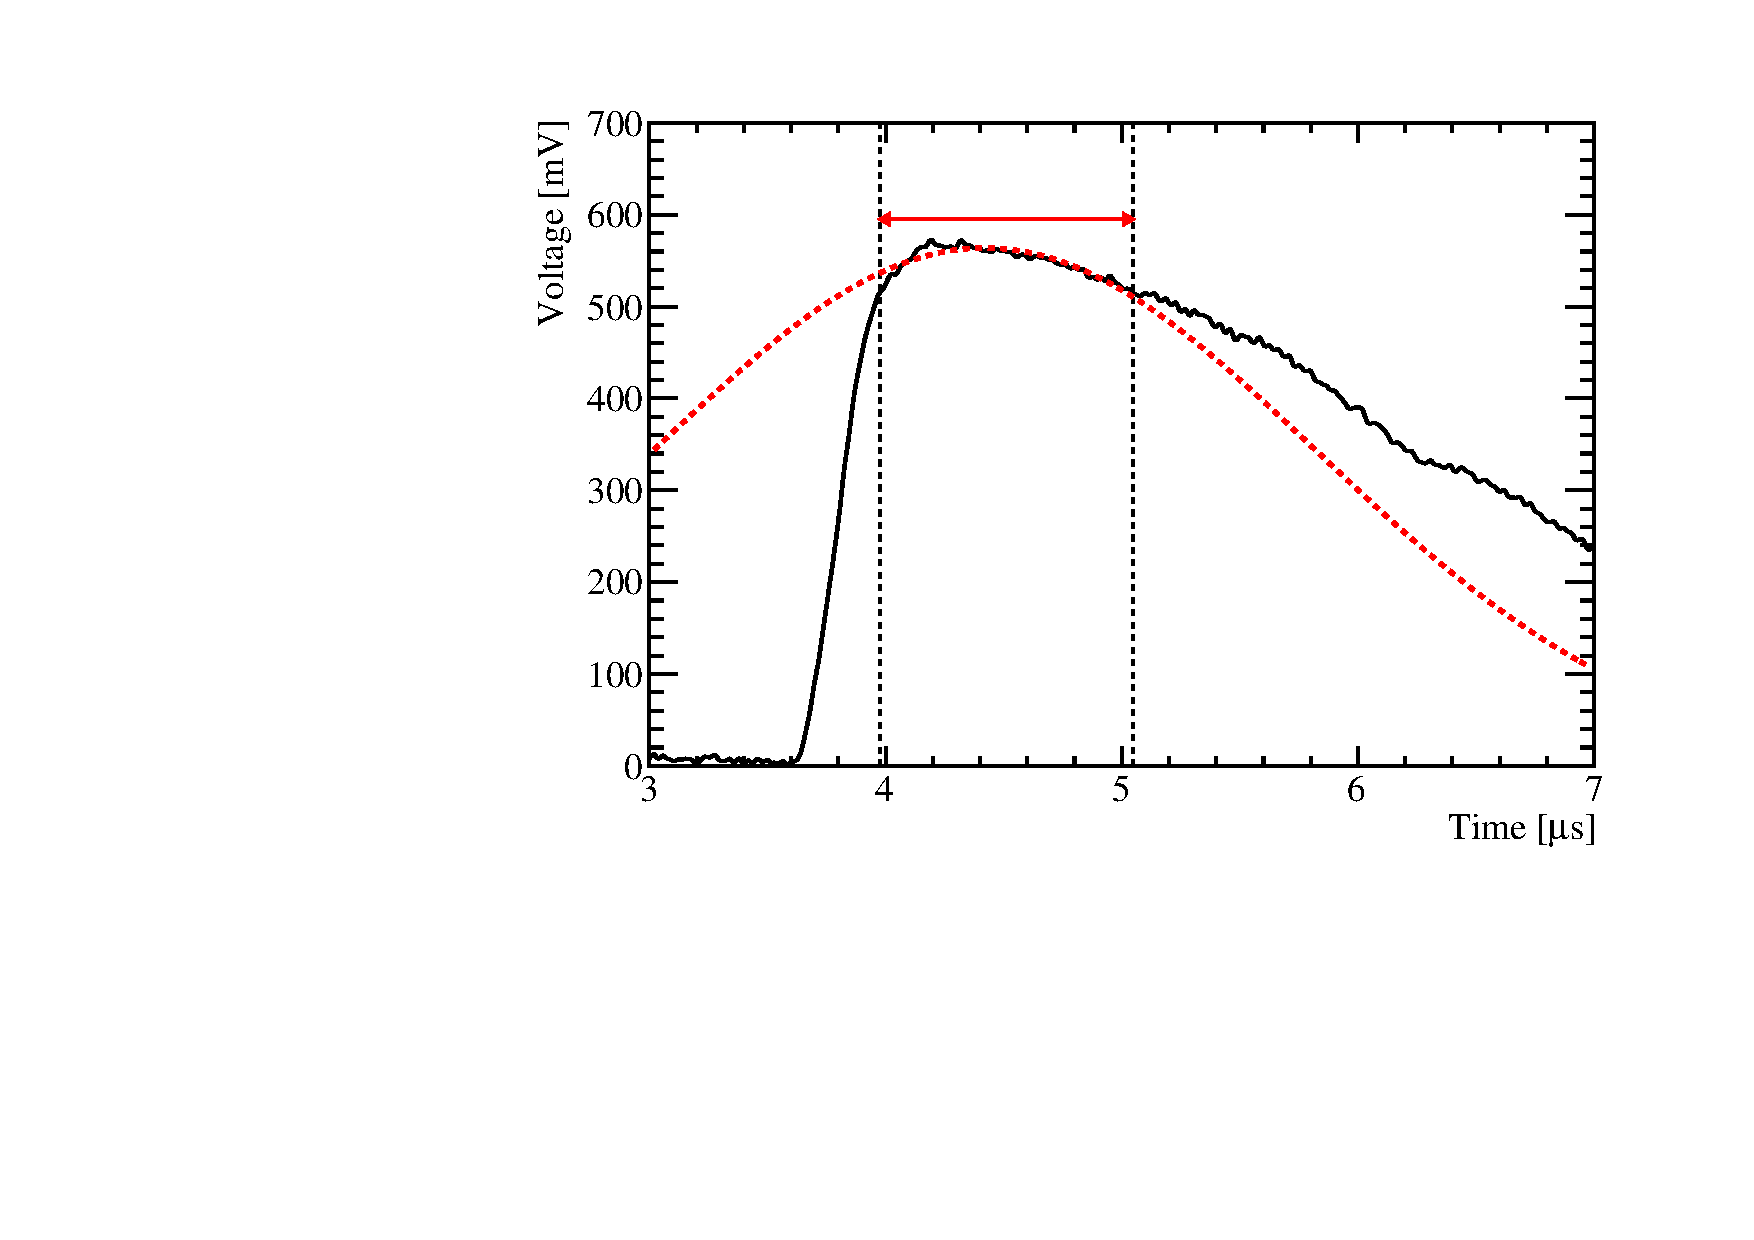
\includegraphics[width=0.5\textwidth]{CLICdpVertex/Plots/HV-CMOS/Frames/PulseShape01000FittingVoltage.pdf}}\hfill

\caption[Analysis of HV-CMOS voltage as a function of time for pulses created by radioactive strontium 90 source.]{Analysis of HV-CMOS voltage as a function of time for pulses created by radioactive $\text{Sr}^{90}$ source.}

\label{fig:pulseshapeanalysis}
\end{figure}

The pulse height was taken as the mean of a Gaussian fit to the peak of the HV-CMOS output signal, defined as the section of the signal above 90\% of the maximum recorded voltage change.  The application of a Gaussian fit provides a more robust metric for categorising the pulse height, which is less dependant on fluctuations in the voltage.  The rise time was calculated as the time taken for the signal to go from 10\% to 90\% of the maximum recorded voltage change.  This definition similarly makes the rise time metric more robust against fluctuations in the voltage.  Examples of the calculation of these metrics for a representative pulse are shown in figure \ref{fig:pulseshapeanalysis}.

For each device the HV-CMOS pulse output was recorded for 15 pixels running along one edge of the 64 $\times$ 64 matrix; in the subsequent analysis the data for all 15 pixels is combined.

%========================================================================================

\subsubsection{Results -  Rise Time vs Pulse Height}
\label{sec:resultsrisetimepulseheight}
The mean rise time as function of pulse height is shown in figure \ref{fig:risetime}.  This was determined by binning the events in terms of pulse height and determining the mean rise time for events in each of those bins.  The pulse height was binned using a bin width of 4 mV ranging from 0 to 700 mV.  At least 100 measurements per pulse height bin were used for the calculation of the average rise time.  The error bars on this figure show the standard error in the mean rise time.  

\begin{figure}
\centering
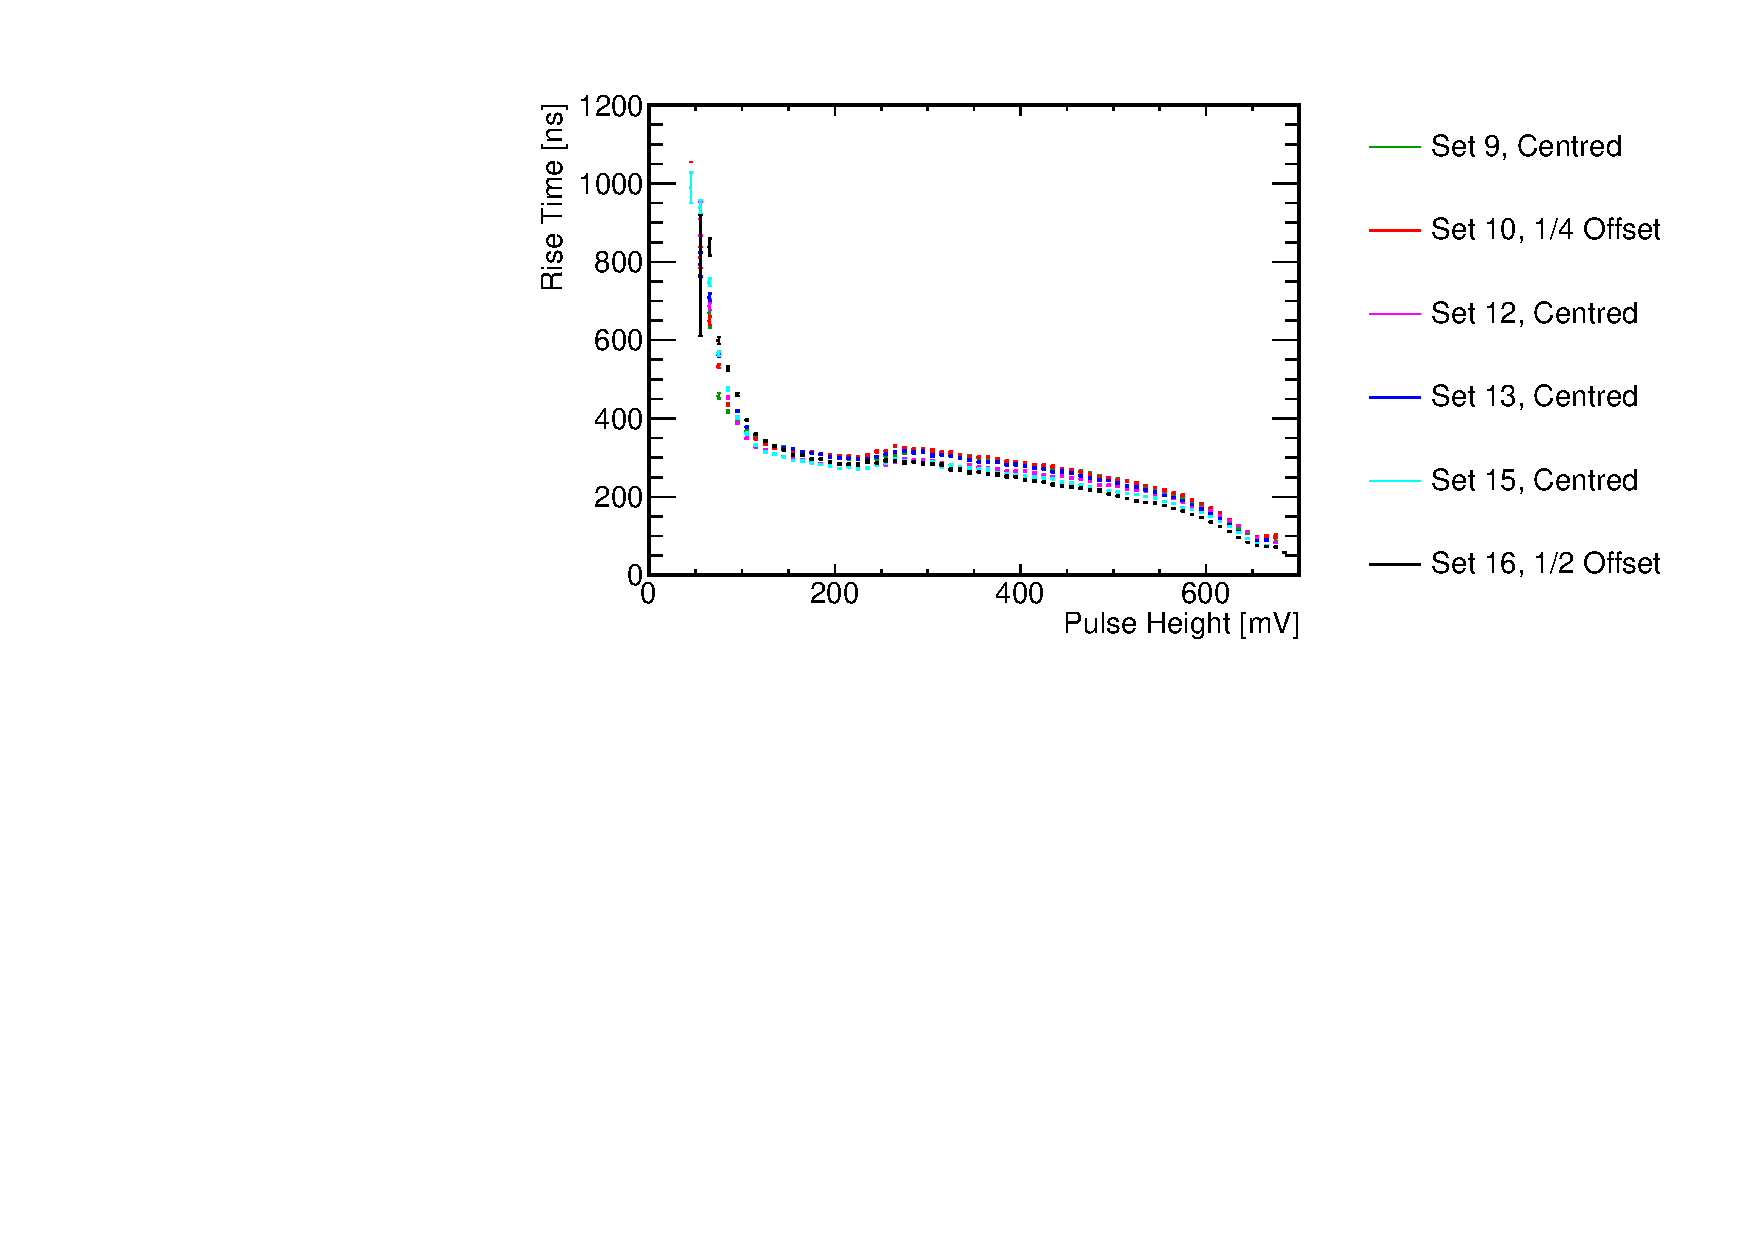
\includegraphics[width=1.0\textwidth]{CLICdpVertex/Plots/RadSourceAnalysis/AllSETs_RiseTime_PulseHeight.pdf}
\caption[HV-CMOS voltage rise time as a function of pulse height.]{HV-CMOS voltage rise time as a function of pulse height. CAN THE FRACTIONS BE MADE THE SAME SIZE AS THE REST OF THE TEXT? }
\label{fig:risetime}
\end{figure}
 
The data in figure \ref{fig:risetime} shows that the rise time for the HV-CMOS front-end is approximately 300~ns across all samples, and that this is largely independent of pulse height for all but the smallest signals. For very small pulse heights ($< 100$ mV) rise times are significantly larger, suggesting that the deposited charge takes a longer time to be collected. This may be due to charge transport via diffusion rather than drift, giving a large increase in the time for the signal charge to be collected. At large values of deposited charge (higher output voltage), a gradual reduction in the rise time is observed, as expected for higher charge deposits. The similar characteristics for all samples makes the comparison of the different misaligned samples more straightforward, as the intrinsic HV-CMOS performance can be seen to be the same. The same must also be true of the CLICpix ASICS, which is indeed the case as the results in section \ref{testpulsecalibrationresults} show.  

%========================================================================================

\subsubsection{Results -  ToT vs Pulse Height}
\label{sec:totvspulseheight}

Figure \ref{fig:tot} shows the mean ToT measured in the CLICpix as a function of the HV-CMOS output voltage pulse height.  The determination of the mean and error bars for the ToT measurement is identical to that described in section \ref{sec:resultsrisetimepulseheight} for the rise time measurement. 

\begin{figure}
\centering
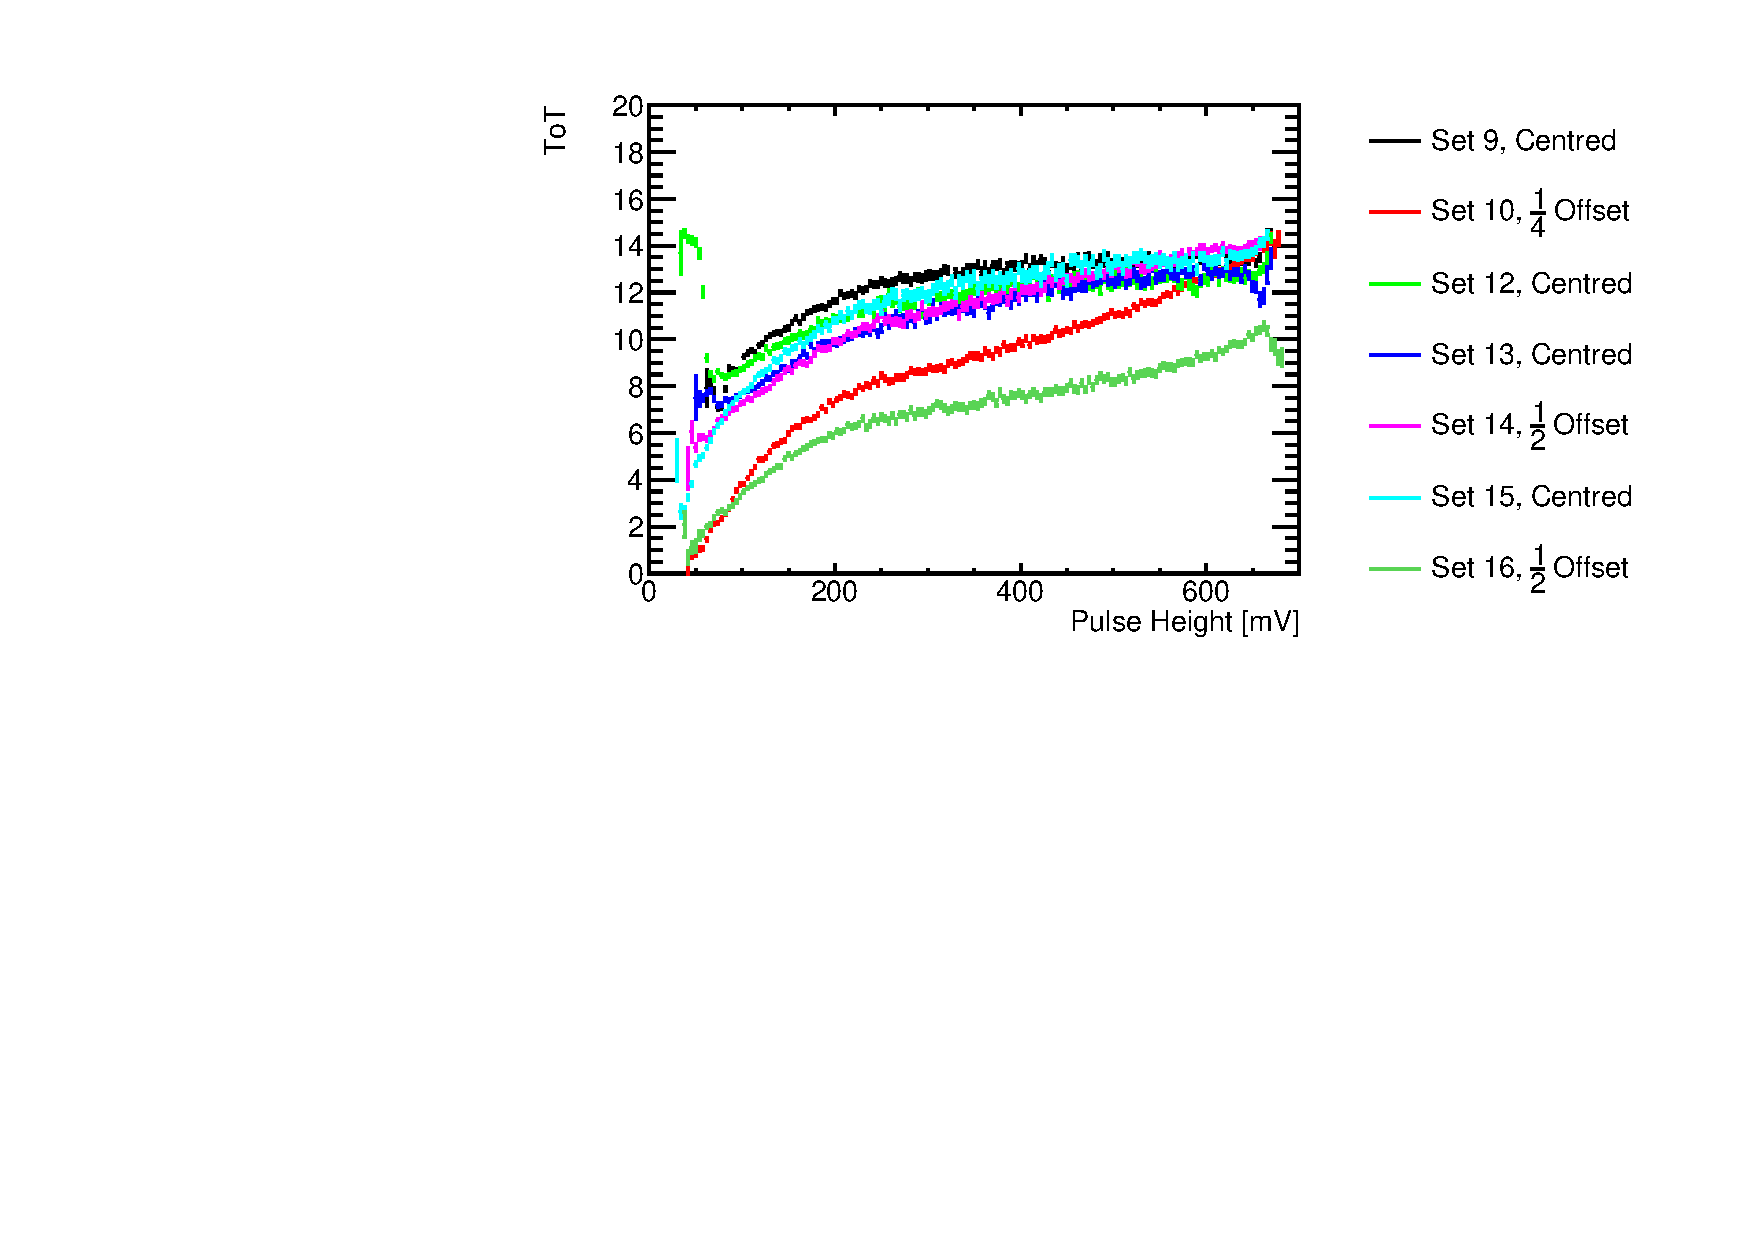
\includegraphics[width=1.0\textwidth]{CLICdpVertex/Plots/RadSourceAnalysis/AllSETs_TargetTot_PulseHeight.pdf}
\caption[CLICpix ToT as a function of HV-CMOS voltage pulse height.]{CLICpix ToT as a function of HV-CMOS voltage pulse height.  SAME COMMENT TO LABELS AND FRACTION SIZES}
\label{fig:tot}
\end{figure}

The distribution of mean ToT versus pulse height shows that for samples where the corresponding coupling pads are centred, the ToT increases with pulse height up to values of approximately 300~mV, and that the mean ToT saturates at $\approx 13$.  It is expected that the $\frac{1}{4}-$ and $\frac{1}{2}-$offset samples should have a lower ToT than the centred samples due to the lower effective capacitance between the HV-CMOS and CLICpix pads.  The greater the offset is, the smaller the effective capacitance to the target CLICpix pad will be, and so the lower the recorded ToT.  This is can be seen when comparing the centred samples to the $\frac{1}{4}-$offset sample and SET 16, the $\frac{1}{2}-$offset sample.  

%========================================================================================
IN GENERAL YOU KEEP FORGETTING TO PUT THINGS IN CONTEXT - WHY CROSS-COUPLING?

\subsubsection{Results -  Cross Couplings}

Due to the capacitive transfer of signal from the HV-CMOS sensor to the readout ASIC, it can be expected that any capacitance between the HV-CMOS pixel pads and the readout pads of neighbouring pixels may give rise to additional unwanted hits. Such cross-capacitancies can be observed in the same manner as the previous measurements, but by considering instead the ToT of the neighbouring CLICpix pixel. This is shown in figure \ref{fig:totcrosscoupling1} for all devices where the pixel pads are centred on each other, and in figure \ref{fig:totcrosscoupling2} for the $\frac{1}{4}-$offset sample and the $\frac{1}{2}-$offset sample, SET 16.  

IN GENERAL USE "SET" INSTEAD OF "SET"

DO YOU HAVE A PLOT SHOWING THE NUMBER OF HITS IN THE NEIGHBOUR? RELATIVE TO THE NUMBER OF HITS IN THE ALIGNED PIXEL? THIS PSEUDO-EFFICIENCY MIGHT BE A BETTER INDICATOR? FOLLOWED BY THESE PLOTS

SO: this part should be rewritten a little. Most likely you have a threshold effect at low pulse heights (not enough charge injected to make a hit, followed by enough to make a hit but just with a "default" low ToT). Then at high pulse heights you start to see a linear rise, which suggests you are now injecting enough charge to have a good correlation. But these are both second order to the point above, of showing that the number of hits in the main peak is N, and in the side peak is M << N (for low coupling).

REMOVE REFERENCES TO SET14!

No correlation between the adjacent pixel ToT and the HV-CMOS pulse height is observed for the samples shown in figure \ref{fig:totcrosscoupling1} for all but the lowest values of pulse height.  The correlation observed at low pulse heights may arise due to the signal $\text{e}^{-}$, which is primarily recorded in the target pixel, depositing a small amount of charge in the adjacent adjacent pixel.  This can happen as the $\text{e}^{-}$ may not be traveling normal to the pixel surface.  However, as this feature is not present in all samples it could indicate a small misalignment exists in the samples showing the correlation.  

There is, however, a strong correlation between adjacent pixel ToT and the HV-CMOS pulse height, shown in figure \ref{fig:totcrosscoupling2}, for SET 16, which is one of the $\frac{1}{2}$ offset samples.  This distribution is almost identical to the the target pixel ToT distribution as a function of HV-CMOS pulse height, which is what would be expected given an equal signal charge sharing between the two readout ASICs.  This indicates the charge sharing is well understood for this $\frac{1}{2}$ offset sample.   

For the $\frac{1}{4}$ offset sample correlation is present only for low pulse heights as was the case for the centred samples.  However, the mean ToT within the uncorrelated region is centred around $\approx$ 5 units of ToT, which is lower than was observed for the centred samples.  This is due to the offset reducing the total capacitance between the HV-CMOS and CLICpix in comparison to the centred samples and thus reducing the ToT recorded.

Cross coupling was observed in one of the $\frac{1}{2}$ offset samples and, assuming that the other $\frac{1}{2}$ offset sample was manufactured incorrectly, then charge sharing was well understood for these $\frac{1}{2}$ offset samples.  No cross coupling was observed for any of the other samples considered in this analysis.  

THE RESULTS OF THIS SECTION SHOULD BE DISCUSSED AND I SHOULD TAKE A LOOK ONCE YOU HAVE CHANGED THE TEXT AROUND AGAIN.

\begin{figure}
\centering
\subfloat[]{\label{fig:totcrosscoupling1}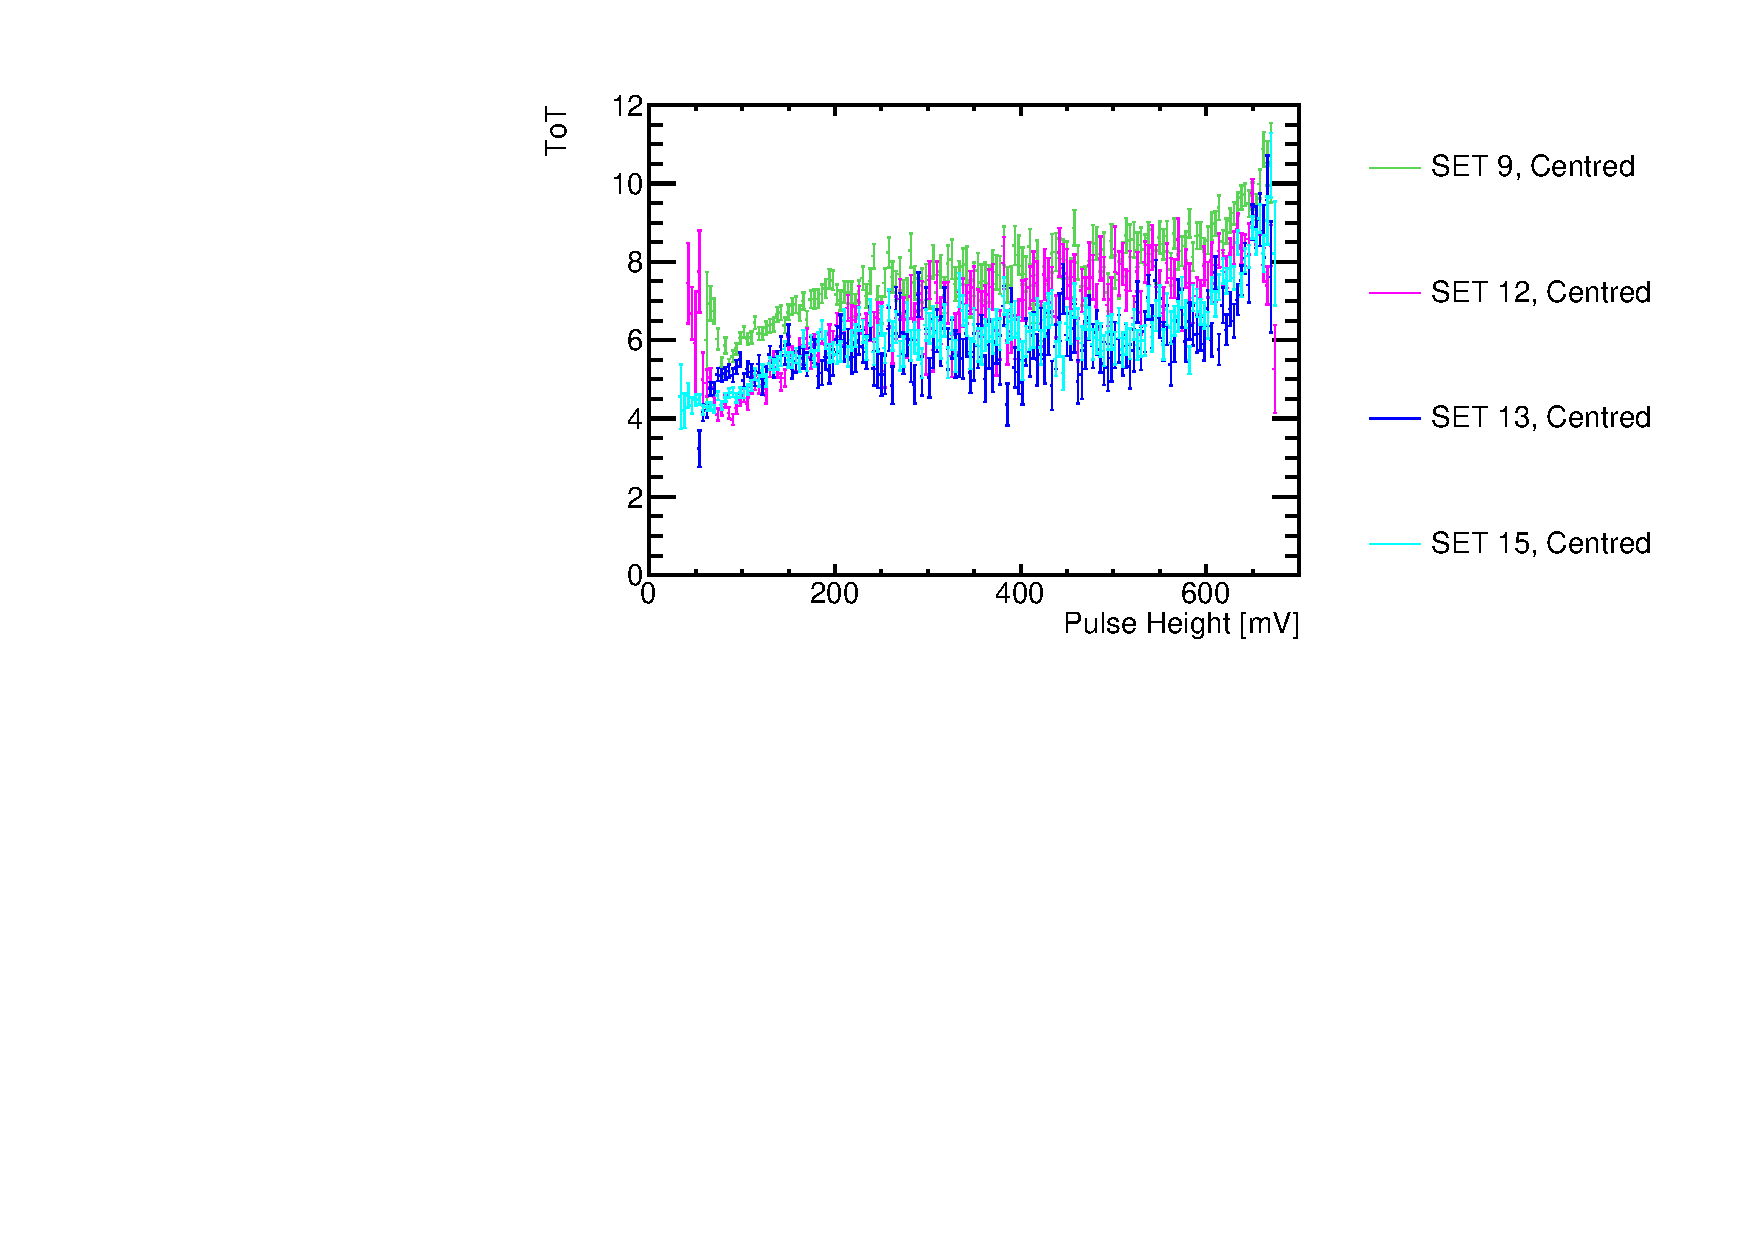
\includegraphics[width=1.0\textwidth]{CLICdpVertex/Plots/RadSourceAnalysis/NoCrossCouplingSETs_Tot_X_PulseHeight.pdf}}\hfill
\subfloat[]{\label{fig:totcrosscoupling2}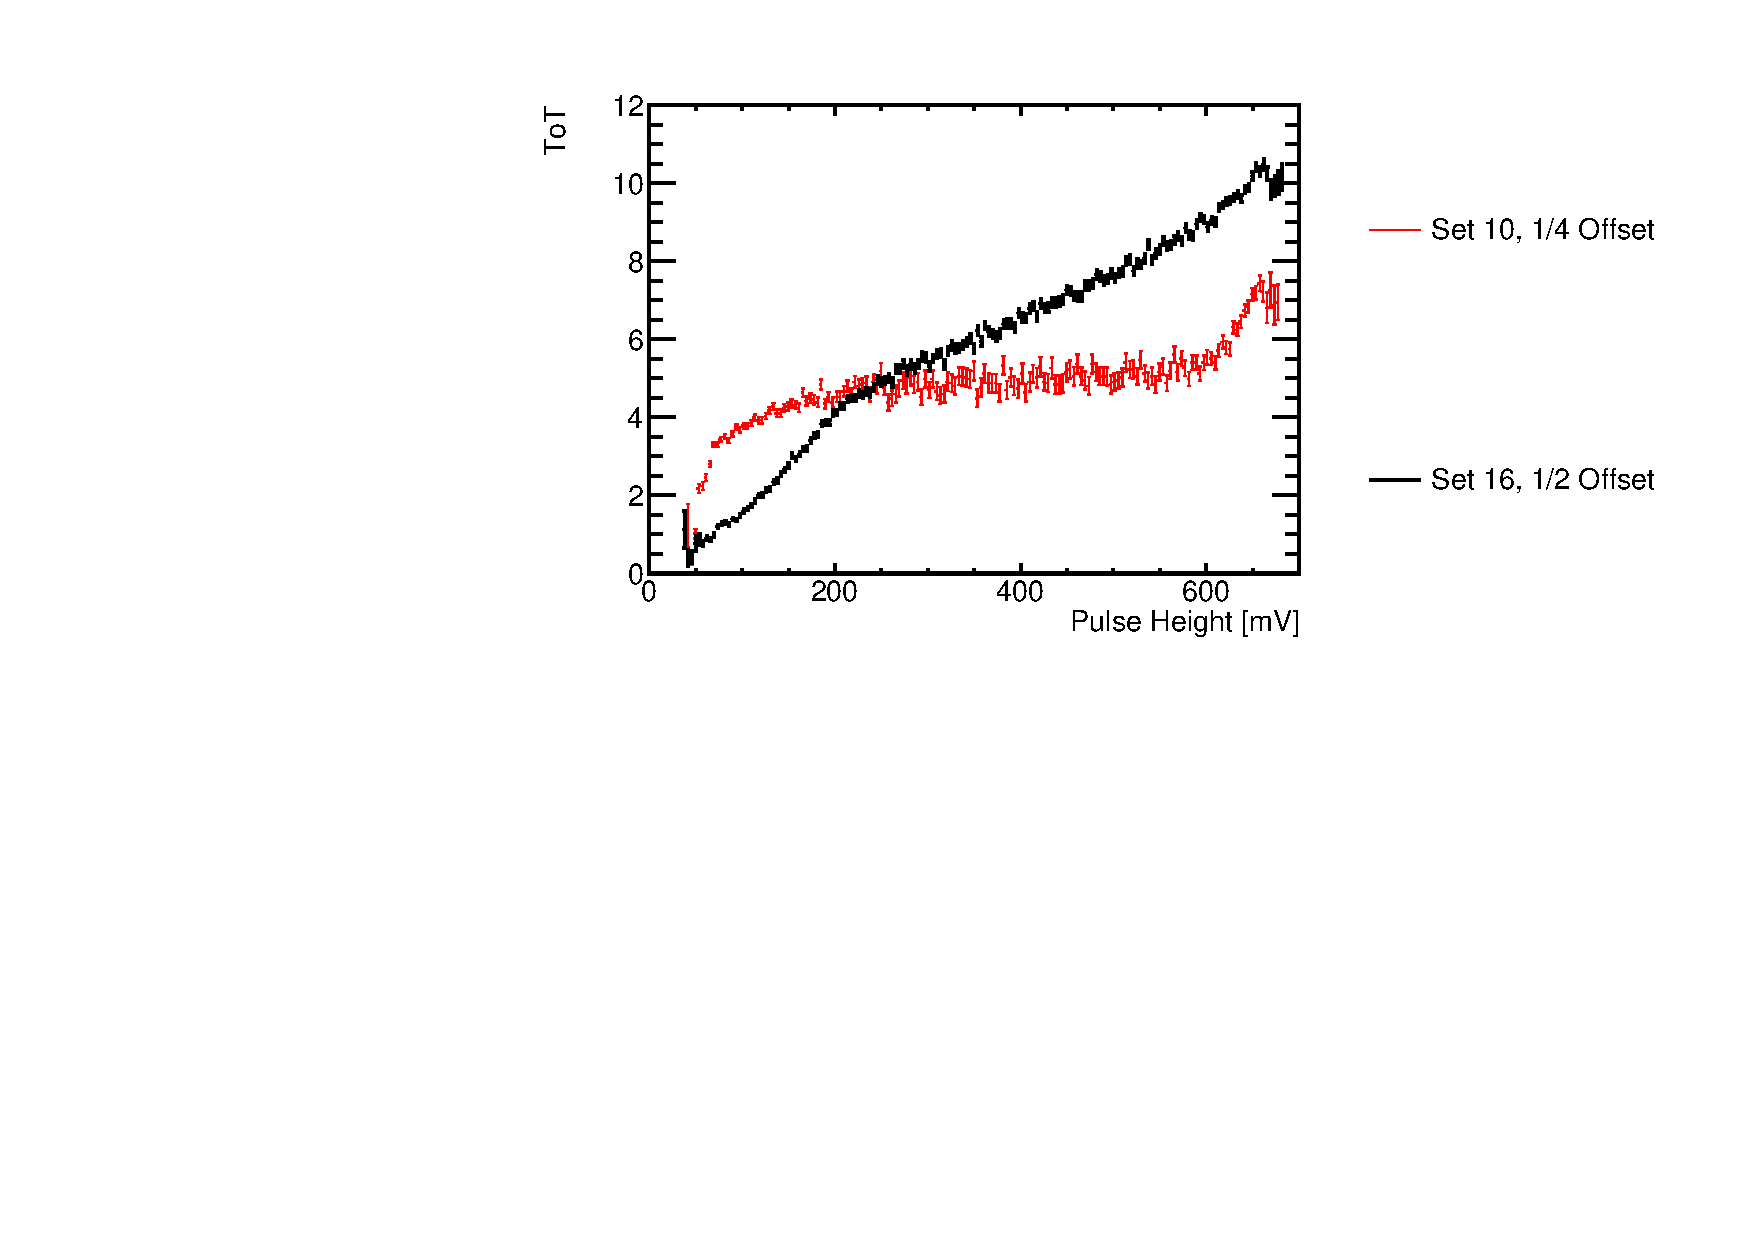
\includegraphics[width=1.0\textwidth]{CLICdpVertex/Plots/RadSourceAnalysis/CrossCouplingSETs_Tot_X_PulseHeight.pdf}}
\label{fig:totcrosscoupling}
\caption[CLICpix ToT on adjacent pixel along the direction of the offset as a function of HV-CMOS voltage pulse height.]{CLICpix ToT on adjacent pixel along the direction of the offset as a function of HV-CMOS voltage pulse height.}
\end{figure}

%========================================================================================

\subsection{Test Pulse Calibration}

%~~~

This measurement focuses upon determining the response of the CLICpix readout chip as a function of the input voltage entering the chip.  The CLICpix readout chip allows for a fixed height voltage pulse to be directly applied at the input of the chip meaning a full calibration of the chip can be performed.  This experiment extends the characterisation of the CLICpix chip beyond what was found using the radioactive source measurements as applying the voltage directly to the CLICpix fully isolates the response of the chip from effects relating to the glue layer.  

%~~~

I WOULD PRESENT A LITTLE MORE "STORY" STYLE, AND NOT SIMPLY AS A LIST OF UNRELATED EXPERIMENTS

In order to understand the charge transfer to the CLICpix, it is important to perform a calibration of the CLICpix front-end response. This was achieved by directly injecting a voltage pulse of fixed height directly into a capacitor held in each pixel, to inject a known quantity of charge. This gives a measure of the performance of the CLICpix independently of the HV-CMOS sensor.  %Due to the construction of the sensor it was not possible to access the HV-CMOS to perform a similar test to isolate its performance.  

%========================================================================================

\subsubsection{Experimental Setup}

In order to prevent any influence from neighbouring pixels during the testpulse measurements the matrix was pulsed in stages, with change injected into 1 out of every 16 pixels while masking the others.  This was repeated 15 more times using different mask configurations until the entire matrix had been sampled. This procedure was repeated 100 times so that the average ToT on a per-pixel level could be recorded.  The pulse height injected into the CLICpix varied from 2 to 180 mV in steps of 2 mV;  an example of the mean ToT plotted against the injected pulse height is shown in figure \ref{fig:testpulseexamplenofit}.  

\begin{figure}
\centering
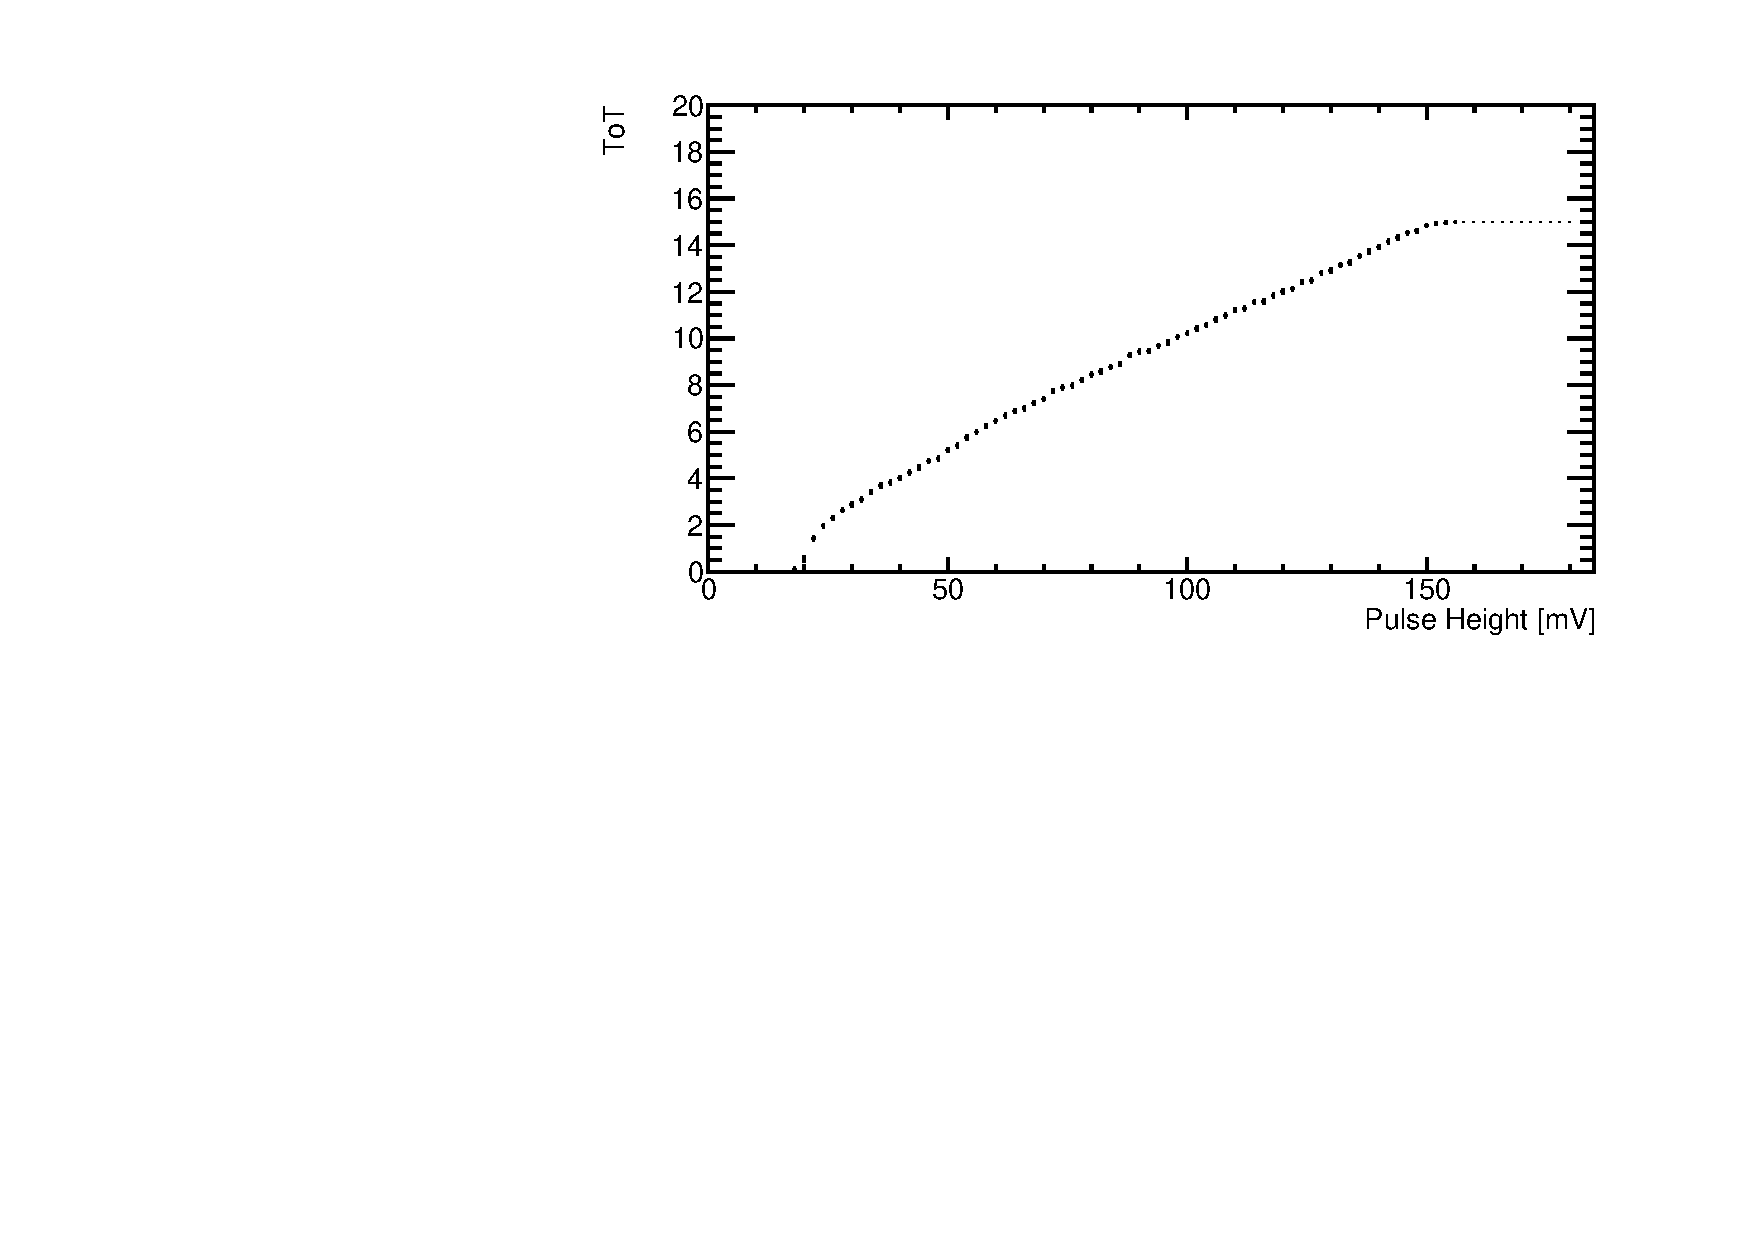
\includegraphics[width=1.0\textwidth]{CLICdpVertex/Plots/TestPulseCalibration/Fits/Set9/ToT_PulseHeight_Set_9_ChipID_001ec0db94b1_Pixel_x0_y0_NoFit.pdf}
\caption[CLICpix ToT as a function of injected pulse height.]{CLICpix ToT as a function of injected pulse height for a single pixel.  The black markers are the mean ToT and the error bars are the standard error on the mean.}
\label{fig:testpulseexamplenofit}
\end{figure}

%========================================================================================

\subsubsection{Analysis}

The functional form of the ToT against pulse height plot is described using a surrogate function as in \cite{AlipourTehrani:2054922}, which is defined as

\begin{equation}
y  = ax + b  - \frac{c}{x-t}
\end{equation}

\noindent where $y$ is the ToT, $x$ is the pulse height and $a$, $b$, $c$ and $t$ are fit parameters.  For large pulse heights the linear relationship dominates while for low pulse heights the inversely proportional term dominates.  $c$ describes the curvature of the graph, while $t$ determines the asymptote below which no signal is detected.  Figure \ref{fig:testpulseexamplefit} shows an example of the application of this fit.  As this function does not describe saturation of the ToT or the region below threshold, the fit is only applied on data points where the mean ToT is greater than 1 and less than 14.75.  

\begin{figure}
\centering
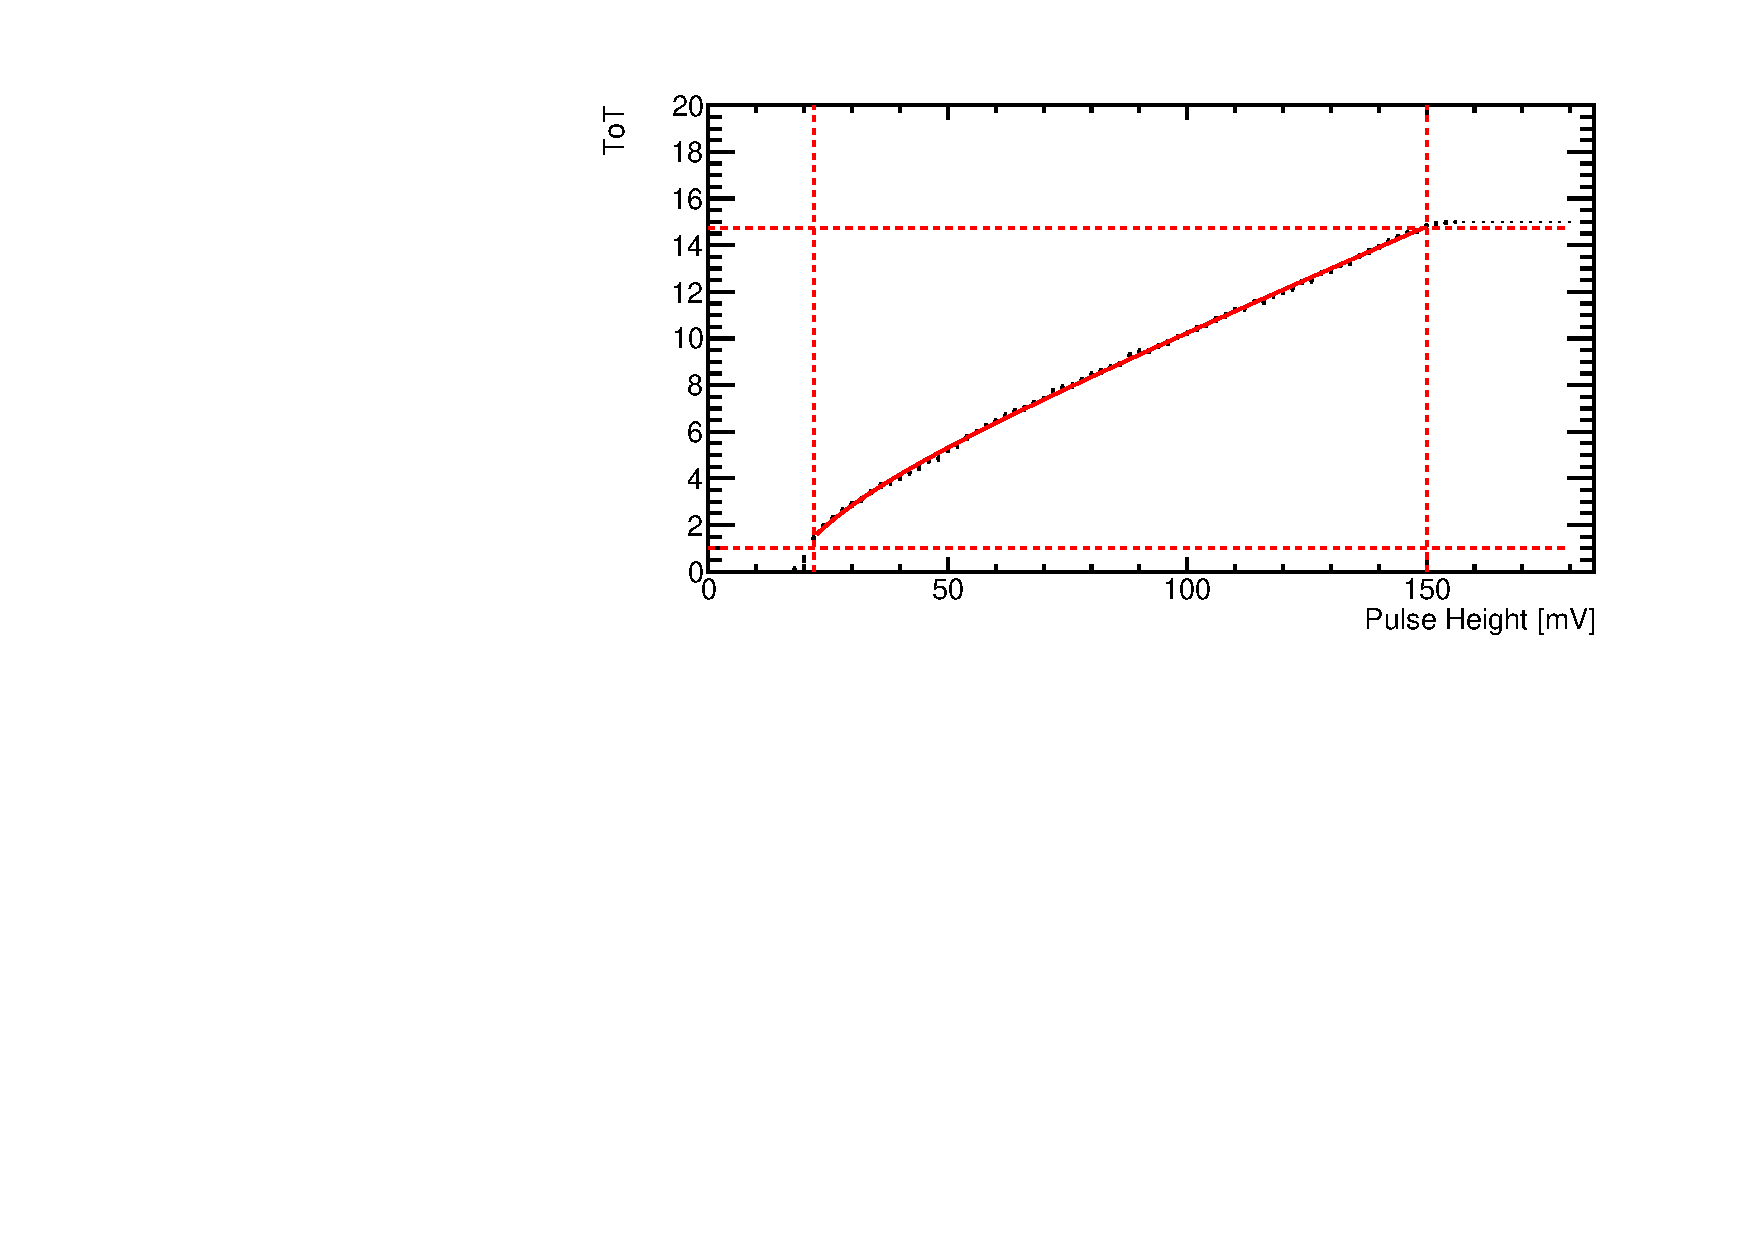
\includegraphics[width=1.0\textwidth]{CLICdpVertex/Plots/TestPulseCalibration/Fits/Set9/ToT_PulseHeight_Set_9_ChipID_001ec0db94b1_Pixel_x0_y0_Fit.pdf}
\caption[CLICpix ToT as a function of injected pulse height.]{CLICpix ToT as a function of injected pulse height for a single pixel.  The black markers are the mean ToT and the error bars are the standard error on the mean.  The solid red line shows the surrogate function fit and the dotted red lines show the range where the fit was applied.}
\label{fig:testpulseexamplefit}
\end{figure}

The application of this fit condenses the information for individual pixels to four parameters.  These parameters can be averaged to categorise the CLICpix response across the matrix.  

%========================================================================================

\subsubsection{Results}
\label{sec:testpulsecalibrationresults}

A known issue withe the design of the CLICpix ASIC is an unwanted feedback capacitance between the discriminator output and amplifier input, leading to a fixed injected charge for each measured hit and operation of the chip at a higher-than-expected threshold. The magnitude of this effect is additionally different for odd and even columns due to the slightly differing physical layouts. This feature can be observed by examining the distribution of the fit parameters;  these are shown for assembly SET9 in figure \ref{fig:fitparams}.  The peak at zero in the distribution of the $a$ and $b$ parameters, $\approx$ 150 in total, correspond to masked pixels in the detector. (CONFIRM THIS!) While the $a$ and $b$ parameters are centred around a single value, indicating a similar response in the linear region of the surrogate function, the $c$ and $t$ parameters are centred around one of two values.  When examining the distribution of these parameters as a function of position on the matrix, shown in figure \ref{fig:fitparams2d} for the same device, it can be seen that the structure is indeed related to the column a given pixel is in.  This feature is present in all devices considered, and the underlying cause will be remedied in the next generation of the CLICpix ASIC.

\begin{figure}
\centering
\subfloat[$a$ parameter.]{\label{fig:fitparams1}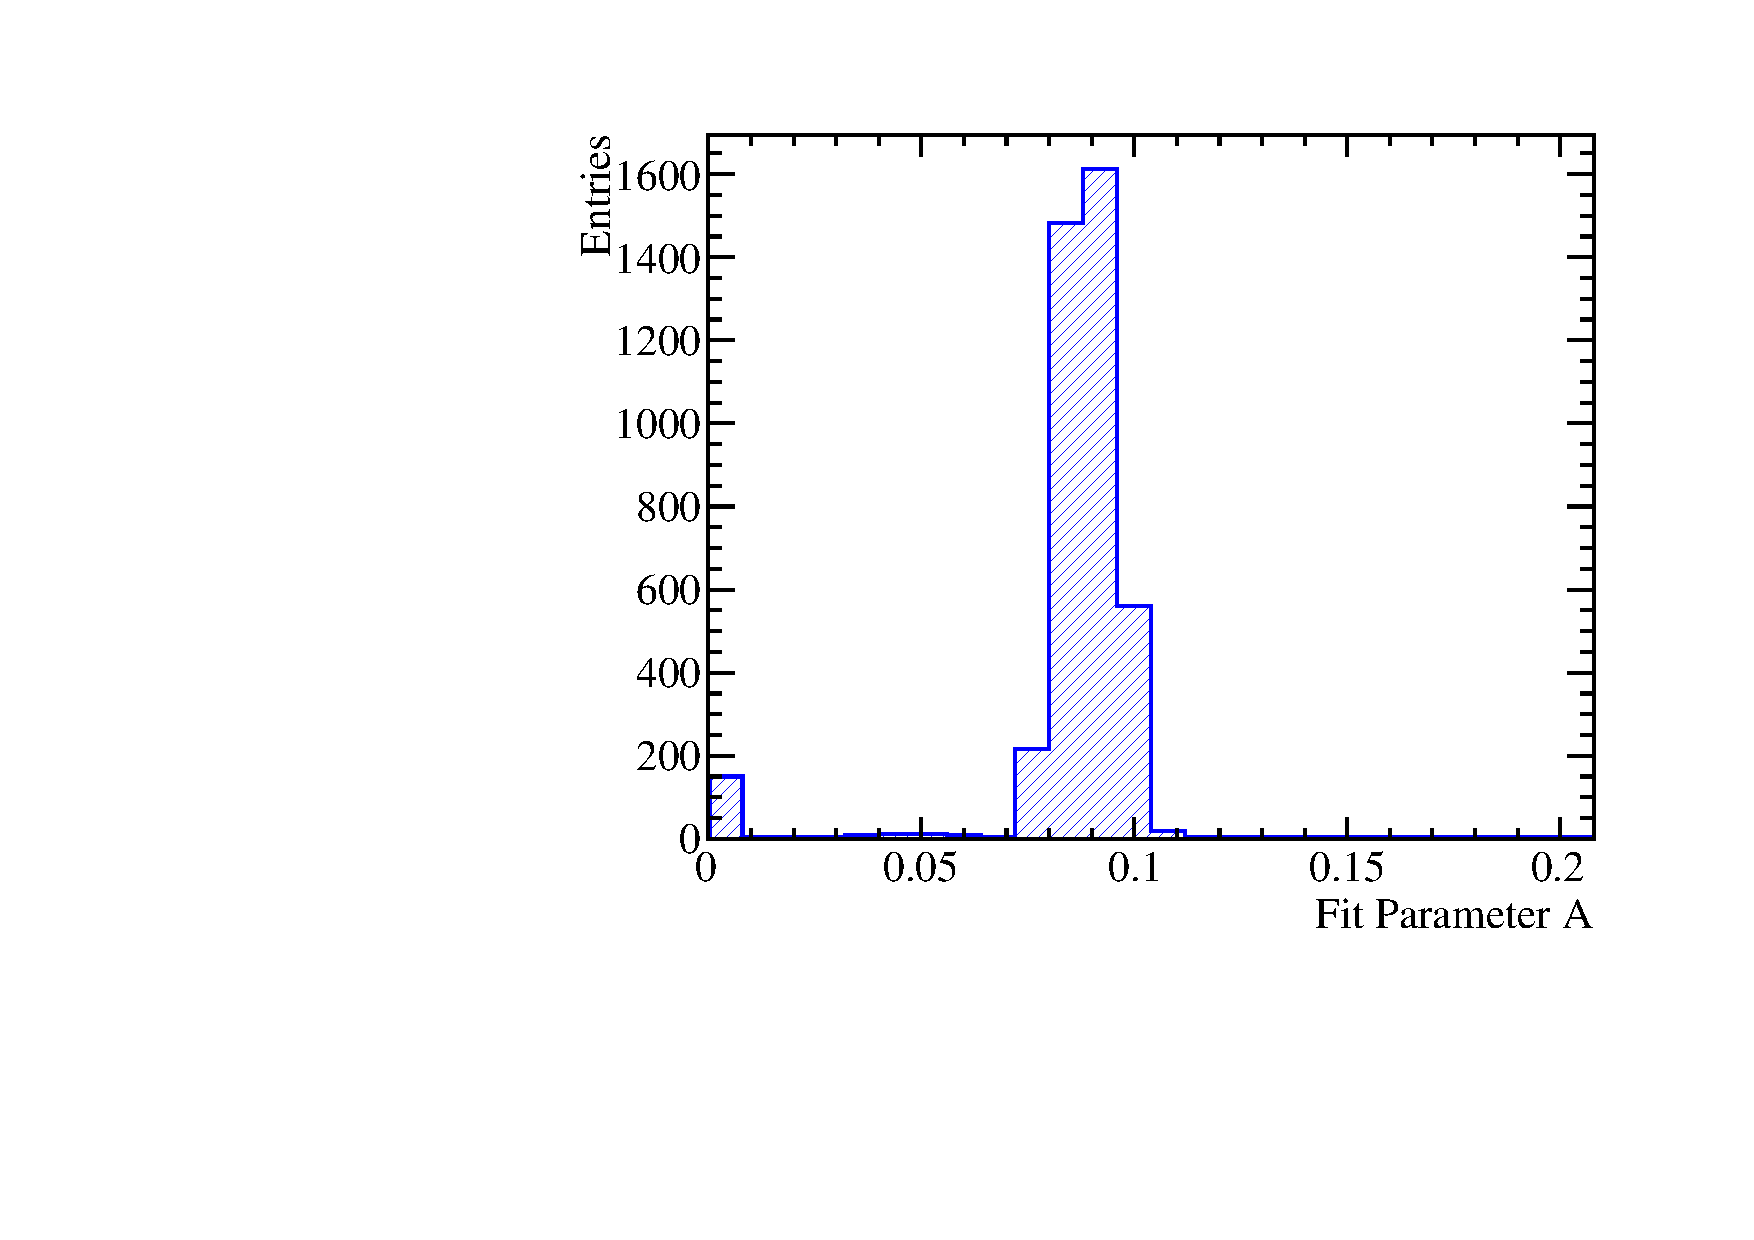
\includegraphics[width=0.5\textwidth]{CLICdpVertex/Plots/TestPulseCalibration/FitParam/OneDHistFitParamA_Set9.pdf}}
\subfloat[$b$ parameter.]{\label{fig:fitparams2}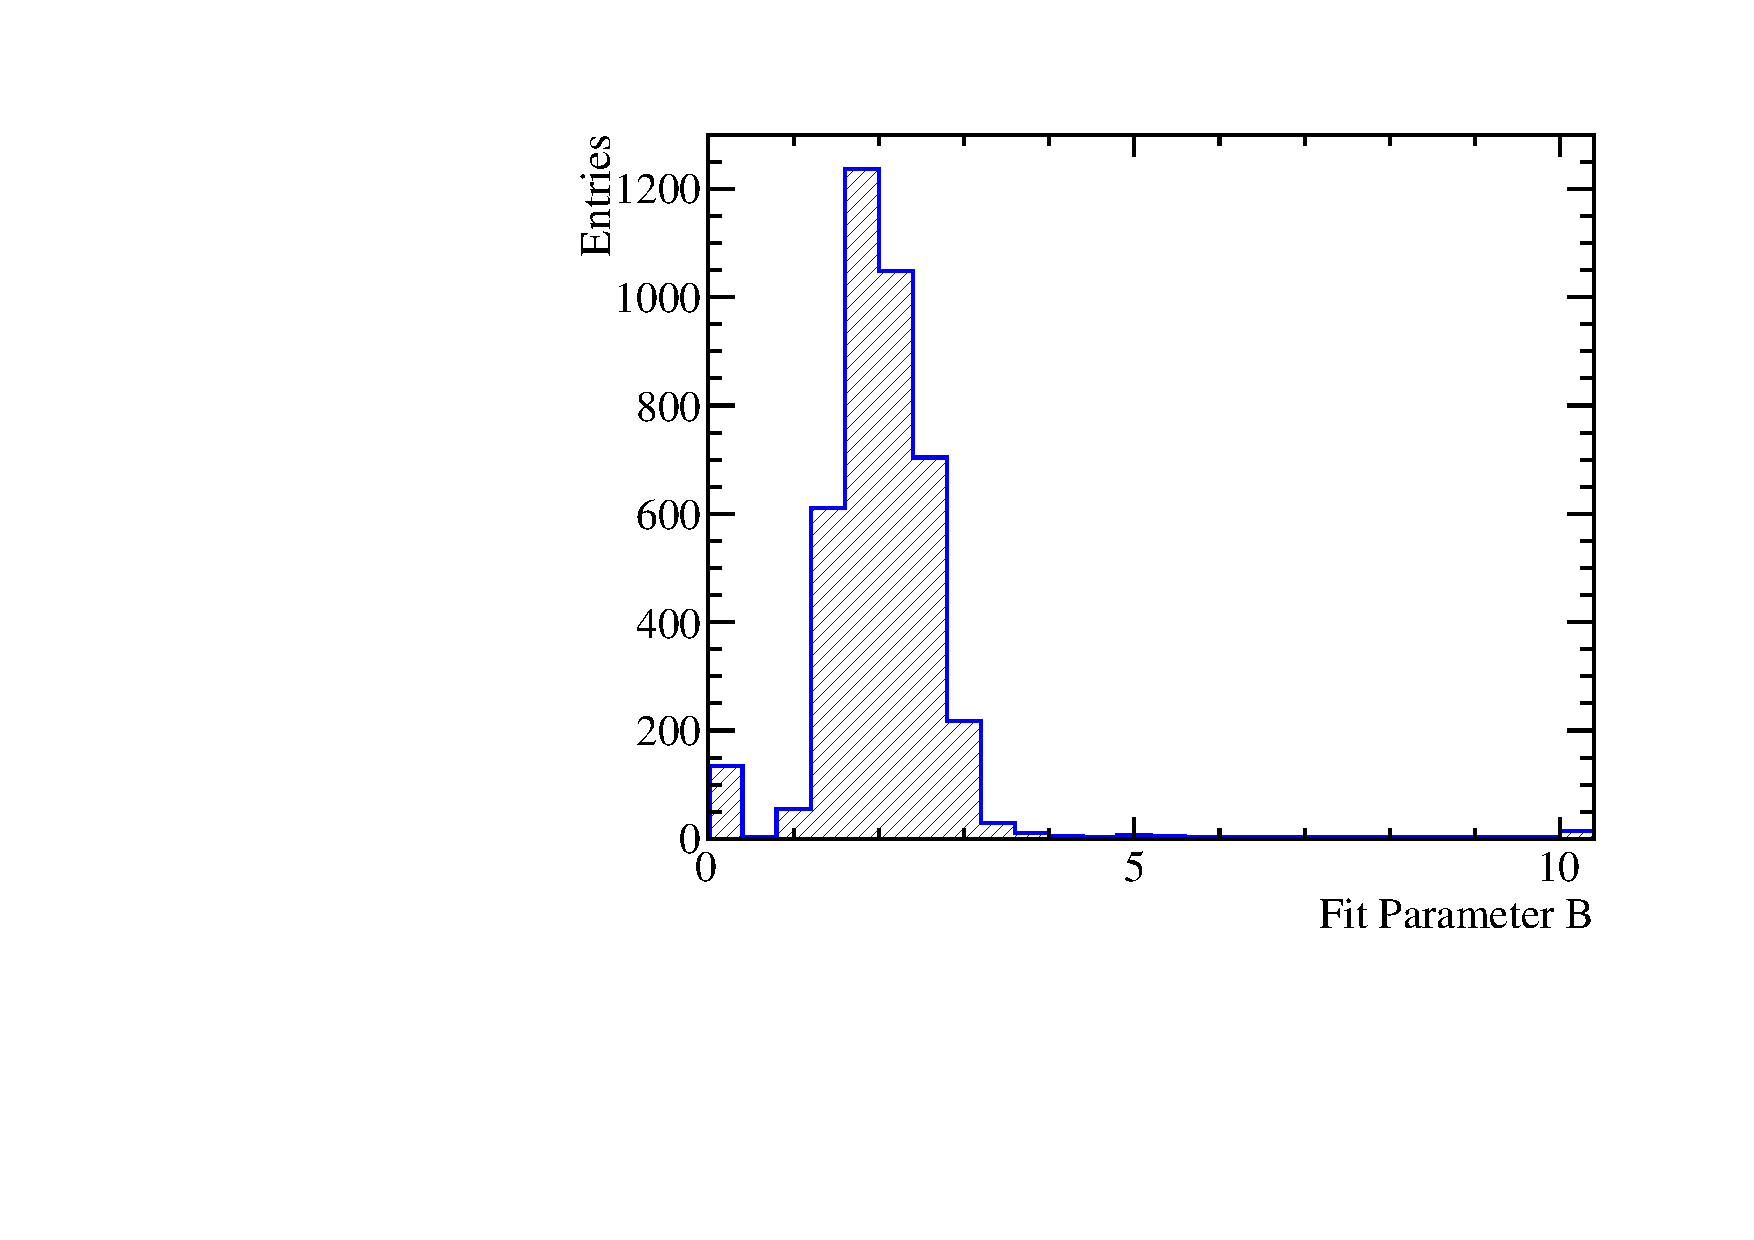
\includegraphics[width=0.5\textwidth]{CLICdpVertex/Plots/TestPulseCalibration/FitParam/OneDHistFitParamB_Set9.pdf}}\hfill
\subfloat[$c$ parameter.]{\label{fig:fitparams3}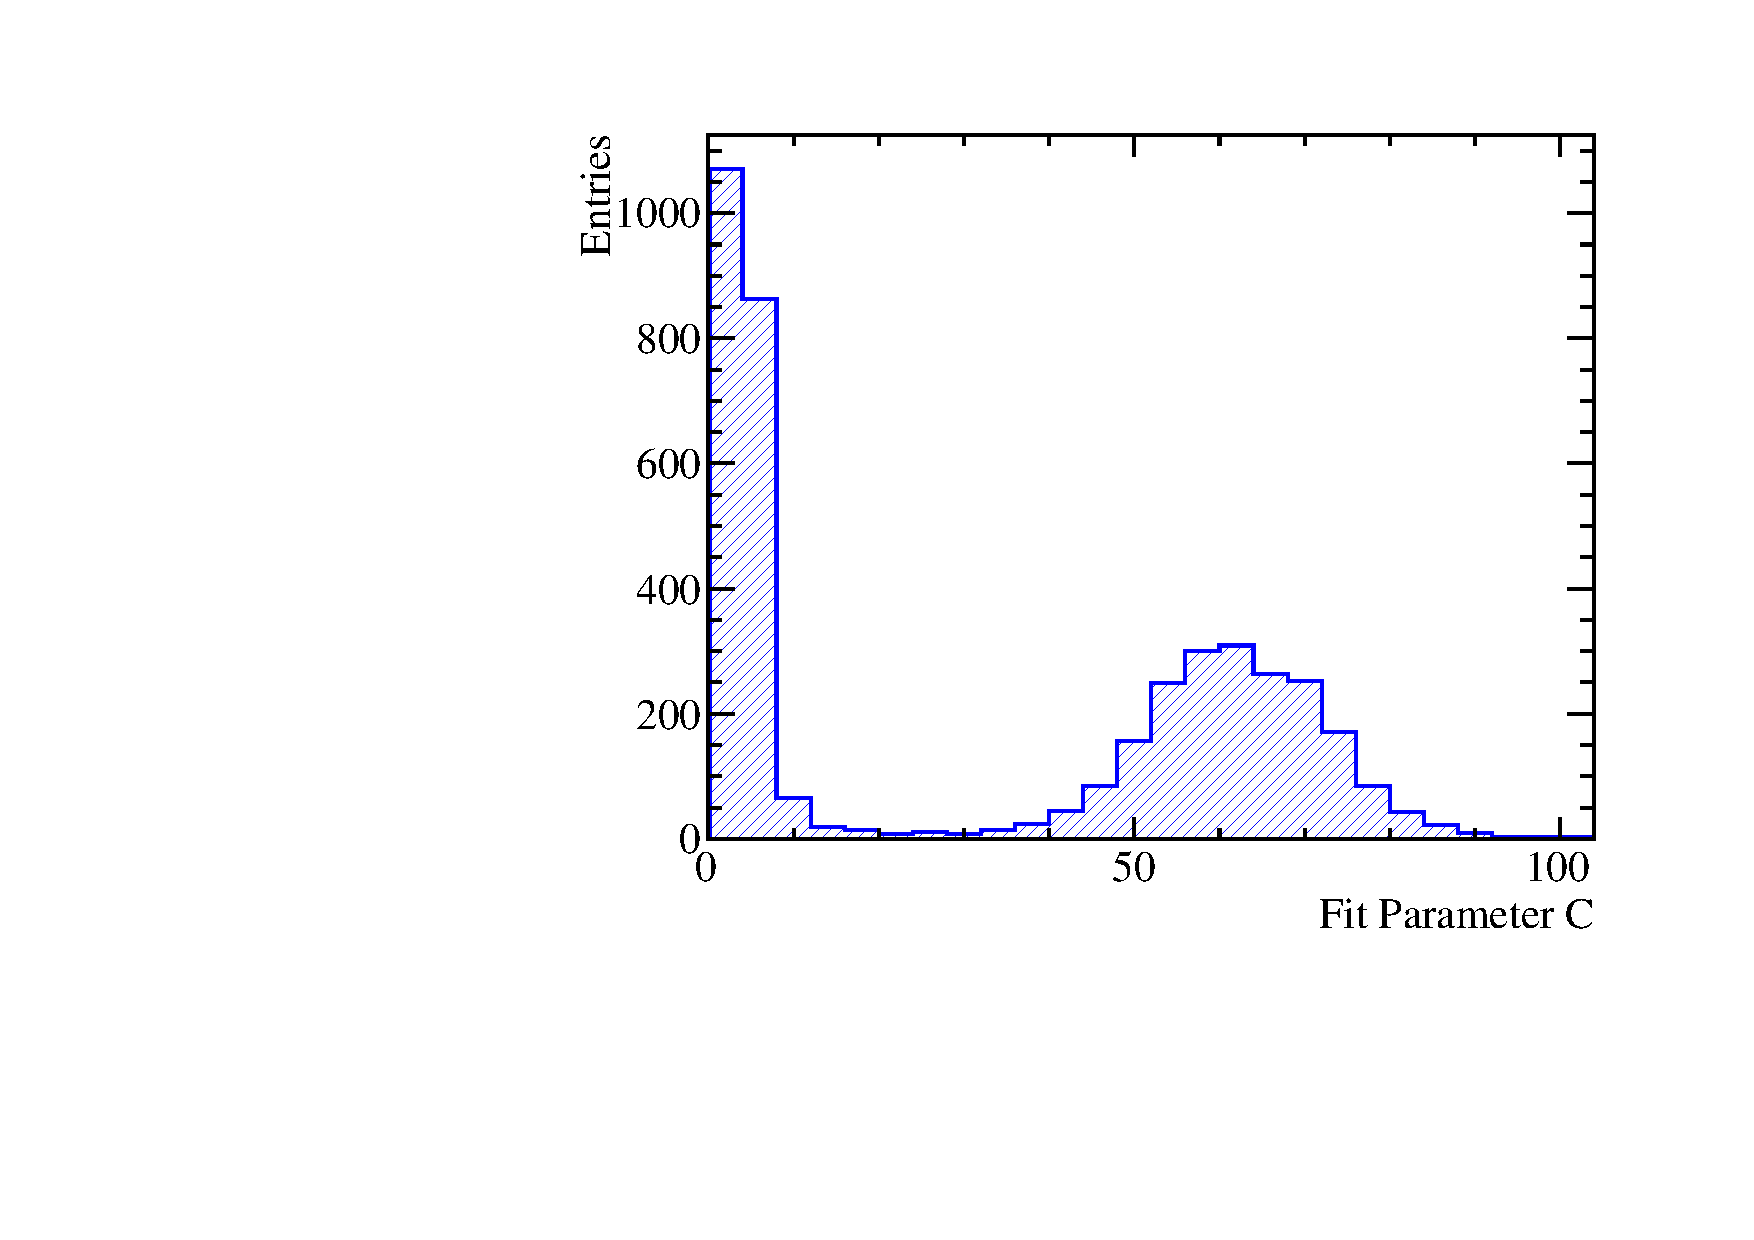
\includegraphics[width=0.5\textwidth]{CLICdpVertex/Plots/TestPulseCalibration/FitParam/OneDHistFitParamC_Set9.pdf}}
\subfloat[$t$ parameter.]{\label{fig:fitparams4}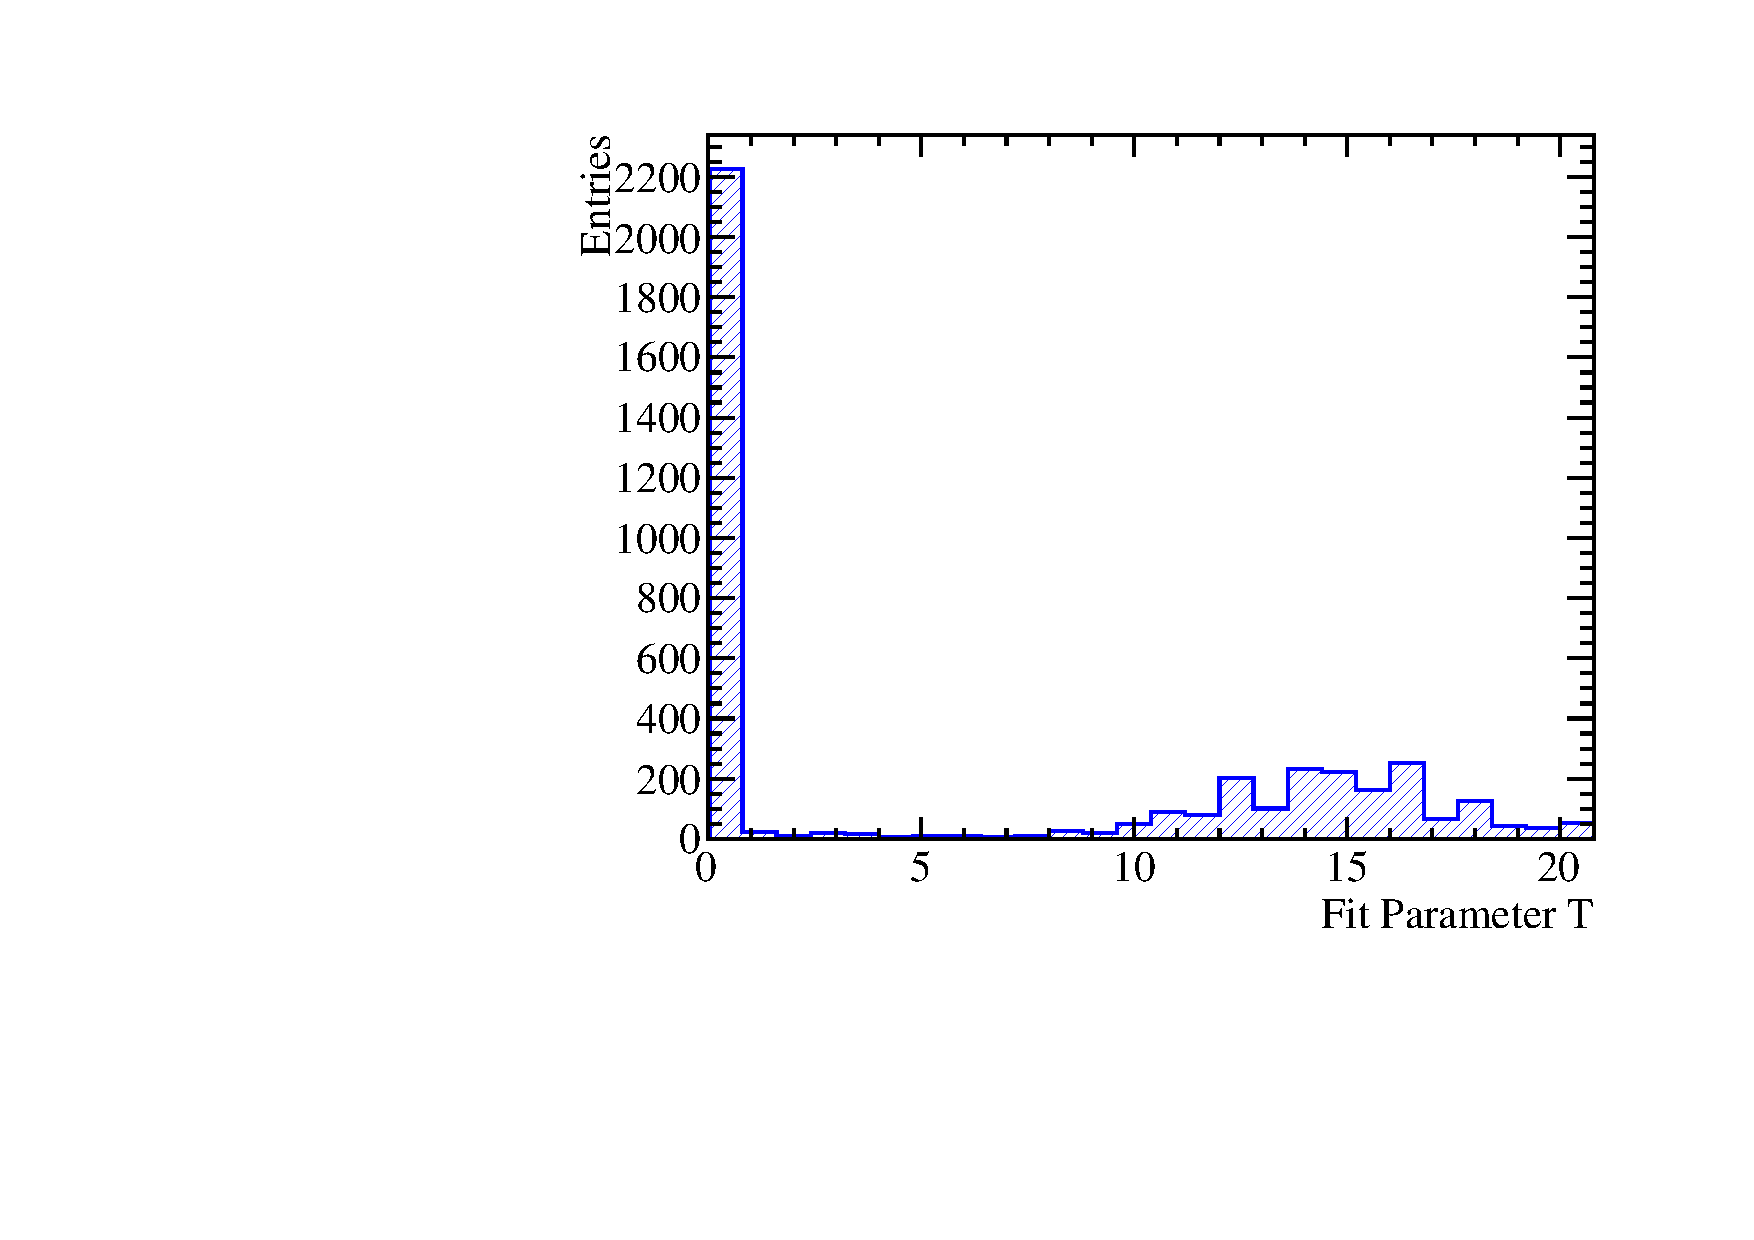
\includegraphics[width=0.5\textwidth]{CLICdpVertex/Plots/TestPulseCalibration/FitParam/OneDHistFitParamT_Set9.pdf}}
\label{fig:fitparams}
\caption[Distribution of surrogate function fit parameters for SET 9.]{Distribution of surrogate function fit parameters for device SET 9.}
\end{figure}

\begin{figure}
\centering
\subfloat[$c$ parameter.]{\label{fig:fitparams2dc}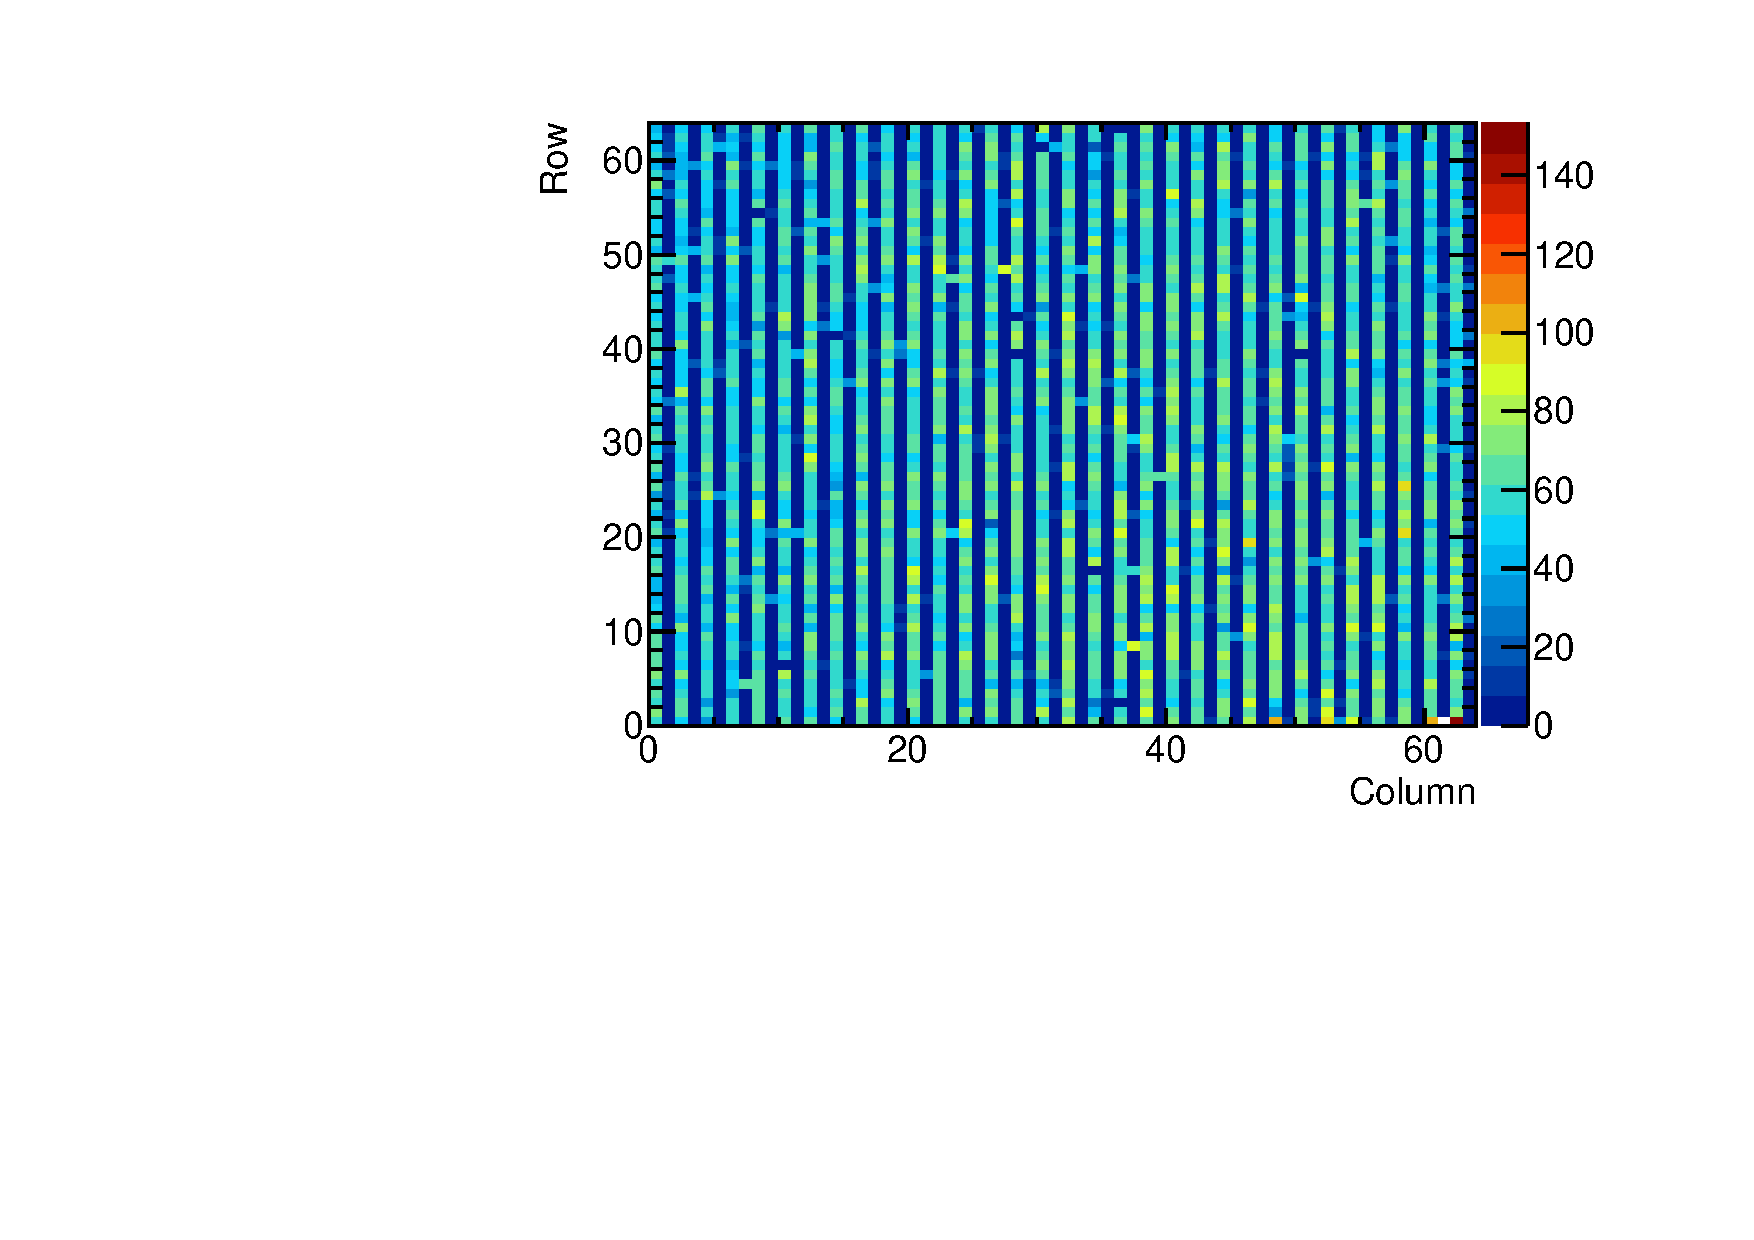
\includegraphics[width=0.5\textwidth]{CLICdpVertex/Plots/TestPulseCalibration/FitParam/FitParamC_Set9.pdf}}
\subfloat[$t$ parameter.]{\label{fig:fitparams2dt}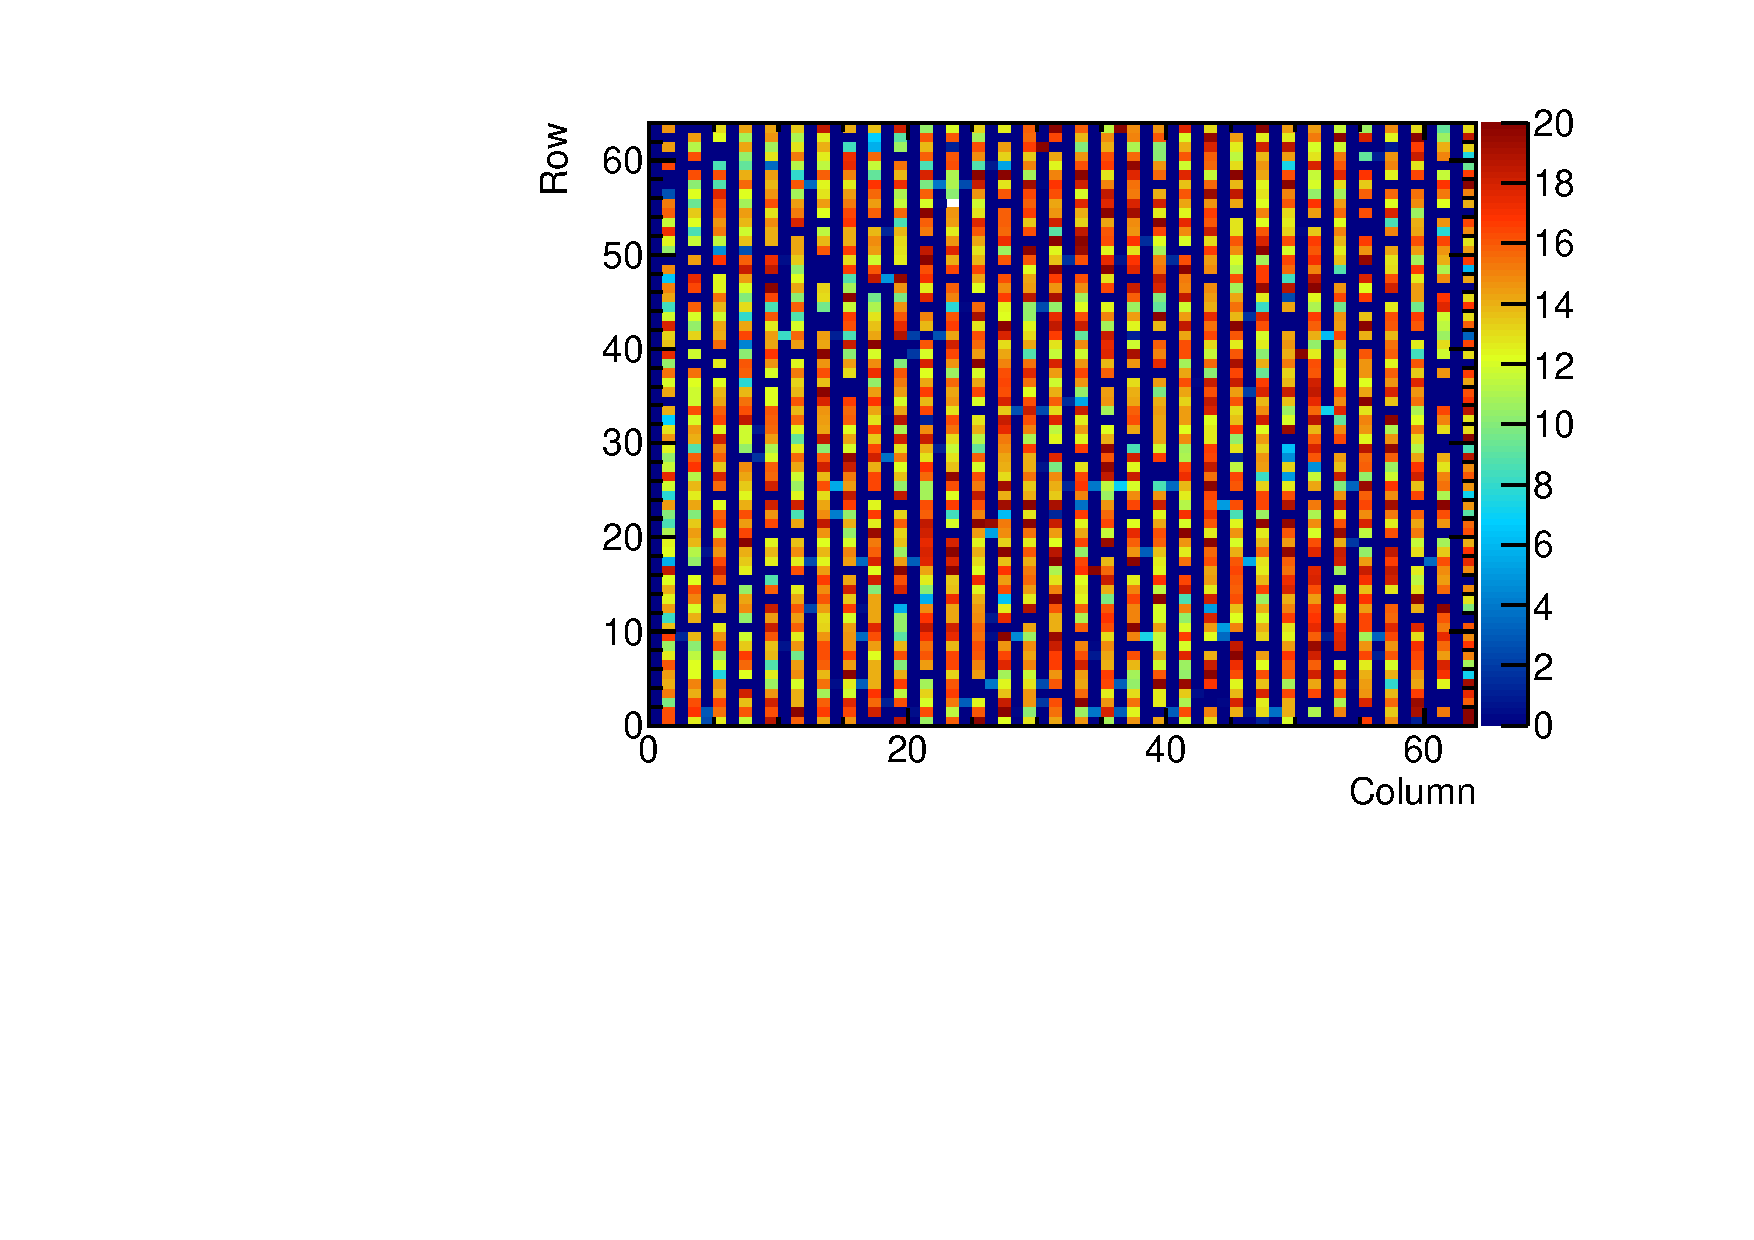
\includegraphics[width=0.5\textwidth]{CLICdpVertex/Plots/TestPulseCalibration/FitParam/FitParamT_Set9.pdf}}
\label{fig:fitparams2d}
\caption[Distribution as a function of matrix position of surrogate function fit parameter $c$ for SET 9.]{Distribution of surrogate function fit parameters $c$ and $t$ for device SET 9.}
\end{figure}

I DONT KNOW WHAT THE FIRST PART OF THE CAPTION IS, BUT IF I HAVE CORRECTED THE SECOND PART (THAT APPEARS IN THE TEXT) PLEASE UPDATE THE FIRST PART IF IT IS RELEVANT AND SHOWN SOMEWHERE!

The matrix-averaged surrogate function fit parameters for all devices can be found in tables \ref{table:clicpixfitparamseven} and  \ref{table:clicpixfitparamsodd}, for the even and odd columns respectively.  The surrogate function using these average parameters as input is shown in figure \ref{fig:testpulsemeanfit}.

REMOVE SET14

\begin{table}[h!]
\centering
\begin{tabular}{ l r r r r}
\hline
Assembly & $a$ & $b$ & $c$ & $t$ \\ 
\hline
SET 9   & $0.0875 \pm 0.0005$ & $2.41 \pm 0.03$ & $5.1 \pm 0.1$ & $12.79 \pm 0.15$ \\
SET 10 & $0.0769 \pm 0.0005$ & $2.58 \pm 0.03$ & $7.5 \pm 0.2$ & $8.02 \pm 0.14$ \\
SET 12 & $0.0725 \pm 0.0005$ & $2.87 \pm 0.04$ & $12.1 \pm 0.3$ & $7.86 \pm 0.22$  \\
SET 13 & $0.0708 \pm 0.0005$ & $2.69 \pm 0.03$ & $16.2 \pm 0.3$ & $6.65 \pm 0.18$ \\
SET 14 & $0.0748 \pm 0.0005$ & $2.57 \pm 0.04$ & $16.0 \pm 1.3$ & $9.89 \pm 0.28$ \\
SET 15 & $0.0856 \pm 0.0005$ & $2.34 \pm 0.03$ & $5.1 \pm 0.2$ & $12.51 \pm 0.13$ \\
SET 16 & $0.0746 \pm 0.0004$ & $2.32 \pm 0.02$ & $13.7 \pm 0.3$ & $6.65\pm 0.16$ \\
\hline
\end{tabular}
\caption[Average fit parameters for even columns of CLICpix sensor.]{Average fit parameters for even columns of the different CLICpix assemblies.}
\label{table:clicpixfitparamseven}
\end{table}

\begin{table}[h!]
\centering
\begin{tabular}{ l r r r r}
\hline
Assembly & $a$ & $b$ & $c$ & $t$ \\ 
\hline
SET 9   & $0.0834 \pm 0.0003$ & $1.72 \pm 0.01$ & $61.0 \pm 0.3$ & $0.25 \pm 0.09$ \\
SET 10 & $0.0759 \pm 0.0002$ & $1.63 \pm 0.01$ & $43.2 \pm 0.2$ & $0.10 \pm 0.02$ \\
SET 12 & $0.0731 \pm 0.0003$ & $1.92 \pm 0.02$ & $51.5 \pm 0.3$ & $0.36 \pm 0.12$ \\
SET 13 & $0.0713 \pm 0.0002$ & $1.72 \pm 0.01$ & $52.5 \pm 0.3$ & $0.18 \pm 0.07$ \\
SET 14 & $0.0754 \pm 0.0002$ & $1.68 \pm 0.01$ & $57.3 \pm 0.3$ & $0.16 \pm 0.03$ \\
SET 15 & $0.0836 \pm 0.0003$ & $1.52 \pm 0.02$ & $52.7 \pm 0.3$ & $0.42 \pm 0.08$ \\
SET16  & $0.0727 \pm 0.0002$ & $1.49 \pm 0.01$ & $50.7 \pm 0.2$ & $0.10 \pm 0.03$ \\
\hline
\end{tabular}
\caption[Average fit parameters for odd columns of CLICpix sensor.]{Average fit parameters for odd columns of the different CLICpix assemblies.}
\label{table:clicpixfitparamsodd}
\end{table}

\begin{figure}
\centering
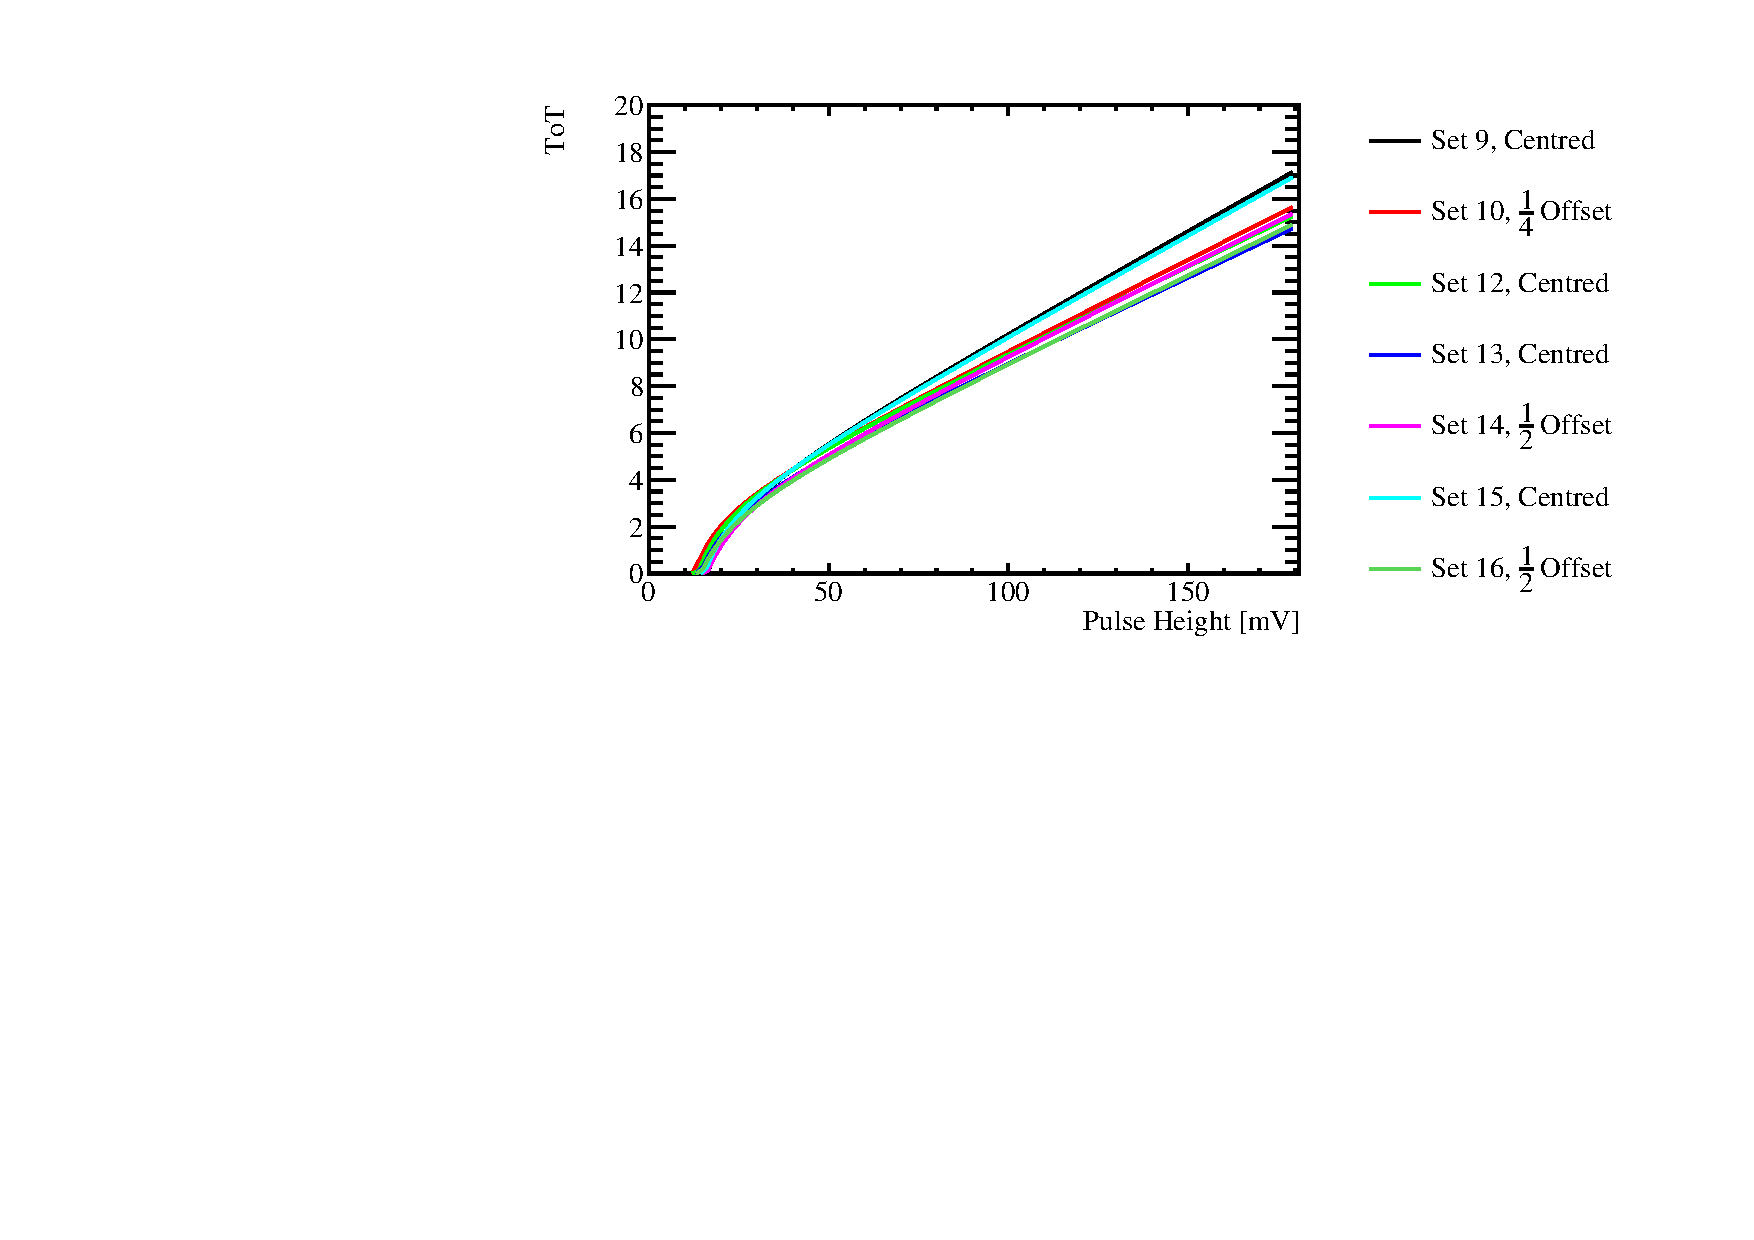
\includegraphics[width=1.0\textwidth]{CLICdpVertex/Plots/TestPulseCalibration/FitParam/AverageToT_vs_InjectedPulseHeight.pdf}
\caption[Fitted CLICpix ToT as a function of injected pulse height averaged across the device matrix.]{Fitted ToT as a function of injected pulse height for all samples, averaged across the device matrix.}
\label{fig:testpulsemeanfit}
\end{figure}

USE A TILDE TO SEPARATE NUMBER AND UNITS IN LATEX, THEN THE UNITS WILL NEVER BE PUT ONTO THE NEXT LINE

As figure \ref{fig:testpulsemeanfit} shows, the response of the CLICpix to the injected pulse height is rather uniform across all samples.  In general, the turn-on pulse height is $\approx$ 10~mV and saturation (i.e. ToT of 15 units) occurs at $\approx$ 150~mV.  For even-numbered columns there is a sharper rise in ToT than for odd-numbered columns due to the different quantity of (unwanted) injected charge. This effect was observed across all devices considered. The uniformity of the sample response ensures that differing effects between the assemblies produced with different misalignments are not due to the response of the CLICpix front end.

%========================================================================================
%========================================================================================

\section{Test Beam Analysis}
\label{sec:testbeam}

%~~~

The lab based measurements have helped to describe many of the characteristics of the devices considered here, however, their use is limited as little information can be deduced about the incoming particles using lab based measurements.  Therefore, to record device efficiencies it is necessary to place the device in a telescope to track the incoming and outgoing particles passing through the device.  Furthermore, the radioactive source calibration cannot be used here as the particles produced by the source would not be of high enough energy to pass through the entire telescope.  This means that it is necessary to use a test beam in conjunction with the telescope to be able to full quantify the device characteristics.

%~~~

AGAIN, BETTER INTRO? Describe a bit why we have to do testbeams, efficiency measurements, etc. Try not to present it in this detached "we have performed an experiment" - there is some reasoning behind this! 

This sections describes the performance of the devices when placed under real experimental conditions at the CERN test beam area.  

%========================================================================================

\subsection{Test Beam Setup}

COMBINED WITH ABOVE COMMENT
The overall goal of this experiment was to determine the tracking performance of the capacitively coupled pixel sensors and to see whether the misalignment of the HV-CMOS and the CLICpix changes the performance.  To that end the samples were mounted on a telescope and placed in a test beam to determine the efficiency, defined as the ratio of number of recorded tracks passing through device to the actual number of tracks passing through device, of the samples.  

These test beam experiments were carried out in August and September 2015 on the H6 beam line in the CERN SPS North Area.  The beam consisted of positively charged hadrons of momenta 120 GeV/c.  Mean particle rates of 500 kHz/cm$^{2}$ were observed during the 4.8 s spills at intervals of 25 s.  \textcolor{red}{Is this data correct?}.

AGAIN, MAYBE EXPAND THIS. You don't really explain why you need a telescope, or what it really is/is used for. Something like "in order to reconstruct the particle trajectory, several planes of detectors are used to..." etc.

During this experiment the samples mounted on an EUDET/AIDA telescope \cite{Rubinskiy:2000287}, which consists of six planes sensors using the Mimosa pixel technology.  This telescope provides a resolution of 1.6 $\mu$m on the intercept position between tracks passing through the device and the device under test (DUT) mounted on it.  

%========================================================================================

\subsection{Analysis}
The track position on the DUT is calculated using the measured particle trajectory through the telescope planes.  This is followed by a search around the intercept position on the DUT to find an associated cluster; a region of 75 $\mu$m, or 3 pixels, about the intercept position is used.  For multi-pixel clusters, the cluster position is calculated as the ToT-weighted centre-of-gravity.  As tracks may undergo non-negligible multiple scattering, a $\chi^{2}$ cut is used to remove less precisely reconstructed particles. Pixels identified on the DUT deemed to be noisy were removed from the analysis, along with any tracks intercepting within half a pixel.  A pixel was deemed noisy if it responded at a mean rate greater than 5 $\sigma$ in comparison to the average rate.  Finally, all tracks occurring within 125 $\mu$m of each other were vetoed, in order to reduce the possibility of mis-association of clusters to tracks. 

MAYBE SAY WHY ALIGNMENT IS NECESSARY? IN GENERAL THIS SECTION COULD DO WITH A LITTLE MORE CONTEXT

An alignment procedure was applied to both the telescope planes and the DUT, in order to account for the physical layout of the setup.  The six telescope planes were aligned by producing rough tracks, and then varying the global alignment parameters of each plane in turn, in order to minimise the track $\chi^{2}$. This was performed iteratively until no further gain was observed. After the telescope planes were aligned, the DUT was aligned by varying its alignment parameters in order to minimise the summed square of track residuals over many events.

%========================================================================================

AGAIN A BIT OF CONTEXT.

\subsection{Single Hit Efficiency}
The single hit efficiency, $\epsilon$, is defined as the number of tracks with associated clusters in the CLICpix assembly, $n$, divided by the number of tracks reconstructed through the detector using the telescope, $m$. The errors shown on the efficiency measurements are given by $\sqrt{\frac{\epsilon (1 - \epsilon)}{m}}$, which follows from the variance of $n$ given binomial statistics with mean $\epsilon$.  

CONTEXT

\begin{figure}
\centering
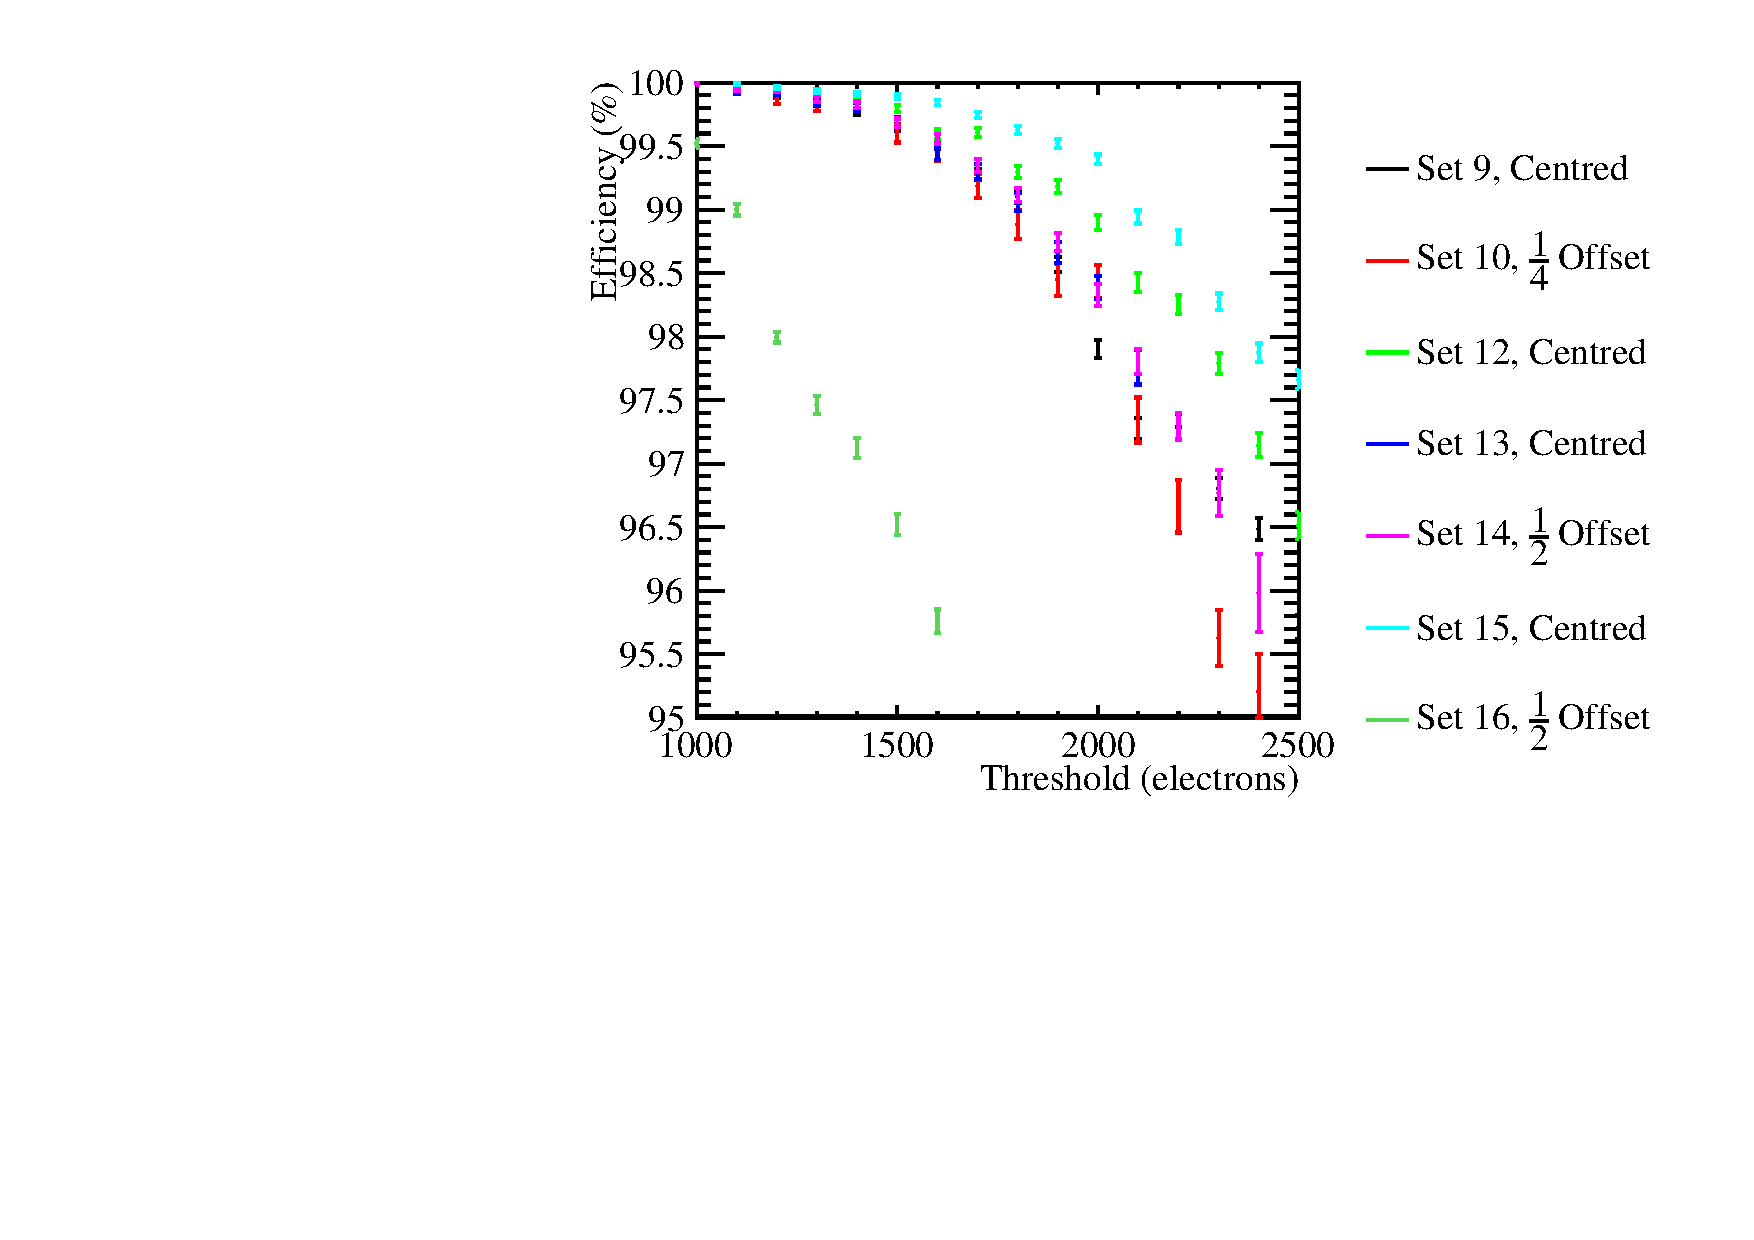
\includegraphics[width=1.0\textwidth]{CLICdpVertex/Plots/TestBeamData/EfficiencyThresholdPlot.pdf}
\caption[Efficiency as a function of threshold.]{Efficiency as a function of threshold.}
\label{fig:efficiency}
\end{figure}

CONTEXT (just in case you missed that ;-))

The efficiency as a function of threshold is shown in figure \ref{fig:efficiency}.  The data indicates that, as expected, for all assemblies the single hit efficiency of the detector decreases when a higher amount of charge is required to generate a signal.  However, it is clear that for the $\frac{1}{2}$ offset sample, SET 16, the efficiency is significantly lower in comparison to the other samples. There is a minor degradation in performance when considering the $\frac{1}{4}$ offset sample, but these results are still comparable to several of the centred samples.  Overall, it can be concluded that manufacturing tolerances up to $\frac{1}{4}$ of a pixel width would not significantly affect performance.    

AGAIN THIS NEEDS EXPANSION. You spent so much time on the earlier section, but now on the results you just say "see figure 1. end.". You can talk a bit more about the lower signal expected by reduced capacitance, etc.

%========================================================================================

\section{Conclusions}


%========================================================================================

  
